%% $Id$
%%
%% TPML 1.0 Benutzerhandbuch
%%
%% Copyright (c) 2005-2006 University of Siegen
%%
%% Written by Christoph Fehling <christoph.fehling@student.uni-siegen.de>, Marcell
%% Fischbach <marcellfischbach@web.de> and Benedikt Meurer <meurer@informatik.uni-siegen.de>.
%%

\documentclass[a4paper,fleqn,latin1,twoside,12pt]{report}

\usepackage{amsmath}
\usepackage{amssymb}
\usepackage{amstext}
\usepackage{german}
\usepackage{ngerman}
\usepackage[latin1]{inputenc}
\usepackage{color}
\usepackage{latexsym}
\usepackage{array}
\usepackage{stmaryrd}

% TP Latex Macros
% General

\newcommand{\Kommentar}[1]{}

\newcommand{\name}[1]{{\text{\it #1\/}}}
%\newcommand{\name}[1]{\mathit{#1}}

%\newcommand{\bfbox}[1]{\mathbf{#1}}

\newcommand{\I}{{\cal I}}

% Proof trees

\newcounter{tree}
\newcounter{node}[tree]

\newlength{\treeindent}
\newlength{\nodeindent}
\newlength{\nodesep}

\newcommand{\refnode}[1]
 {\ref{\thetree.#1}}

\newcommand{\contextcolor}{\color{blue}}



\definecolor{darkgreen}{rgb}{0.1,0.5,0}
\definecolor{redexcolor}{rgb}{0.7,1,0}
%\definecolor{argumentcolor}{rgb}{0.7,1,0}
%\definecolor{bindingcolor}{rgb}{0,0,0.8}
%\definecolor{scopecolor}{rgb}{0.8,0,0}
%\definecolor{holecolor}{rgb}{0.1,0.1,0.8}
%\definecolor{parametercolor}{rgb}{0,0,0.8}


\newcommand{\bindingarrow}{{\color{c905} $\longrightarrow$}}
\newcommand{\argument}[1]{\colorbox{c090}{#1}}
\newcommand{\scope}[1]{\colorbox{c992}{#1}}
\newcommand{\hole}[1]{{#1}}
\newcommand{\parameter}[1]{\colorbox{c905}{#1}}

\newcommand{\resulttypecolor}{\color{darkgreen}}

\newcommand{\resultcolor}{\color{blue}}

\newcommand{\byrulecolor}{\color{red}}

\newcommand{\marked}[1]{\colorbox{redexcolor}{$#1$}}

\newcommand{\smallsteparrow}[1]{\stackrel{\mbox{\scriptsize\byrulecolor (#1)}}{\longrightarrow}}

\newcommand{\byrule}[1]{\hspace{-5mm}\byrulecolor\mbox{\scriptsize\ #1}}

\newif\ifarrows 
\arrowsfalse 

\newcommand{\arrow}[3]
  {\ifarrows
   \ncangle[angleA=-90,angleB=#1]{<-}{\thetree.#2}{\thetree.#3}
   \else
   \fi}

\newcommand{\node}[4]
 {\ifarrows
   \else \refstepcounter{node}
         \noindent\hspace{\treeindent}\hspace{#2\nodeindent}
         \rnode{\thetree.#1}{\makebox[6mm]{(\thenode)}}\label{\thetree.#1}
         $\blong 
          #3 \\ 
          \byrule{#4} 
          \elong$
         \vspace{\nodesep}
   \fi}

\newcommand{\dummyarrow}[3]
  {\arrow{#1}{#2}{#3dummy}}

\newcommand{\dummynode}[2]
 {\ifarrows 
  \else \noindent\hspace{\treeindent}\hspace{#2\nodeindent}
         \rnode{\thetree.#1dummy}{\makebox[6mm]{(\refnode{#1})}}\label{\thetree.#1dummy}
         $\ldots$
         \vspace{\nodesep}
   \fi}

\newcommand{\mktree}[1]
 {\stepcounter{tree} #1 \arrowstrue #1 \arrowsfalse}

\fboxrule=0mm

\newcommand{\cenv}[1]{\fbox{$\begin{array}{|ll|}\hline #1 \\\hline\end{array}$}}


% Special Symbols

\newcommand{\uminus}{\widetilde{\ }}
\renewcommand{\uminus}{-\,}
\newcommand{\nop}{()}


% Im X-Symbol-Manual empfohlen

\newcommand{\nsubset}{\not\subset}
%\newcommand{\textflorin}{\textit{f}}
\newcommand{\setB}{{\mathord{\mathbb B}}}
\newcommand{\setC}{{\mathord{\mathbb C}}}
\newcommand{\setN}{{\mathord{\mathbb N}}}
\newcommand{\setQ}{{\mathord{\mathbb Q}}}
\newcommand{\setR}{{\mathord{\mathbb R}}}
\newcommand{\setZ}{{\mathord{\mathbb Z}}}
\newcommand{\coloncolon}{\mathrel{::}}

% Eigene (k\"urzere) Befehle

\newcommand{\pfi}{\varphi}
\newcommand{\eps}{\varepsilon}
\newcommand{\eval}{\Downarrow}
\newcommand{\pto}{\hookrightarrow}
\newcommand{\emp}{\emptyset}
\newcommand{\sleq}{\subseteq}
\newcommand{\sgeq}{\supseteq}
\newcommand{\sqleq}{\sqsubseteq}
\newcommand{\sqgeq}{\sqsupseteq}
\newcommand{\lub}{\bigsqcup}
\newcommand{\glb}{\bigsqcap}
\newcommand{\lsem}{\llbracket}
\newcommand{\rsem}{\rrbracket}
\newcommand{\impl}{\models}
\newcommand{\step}{\vdash}
\newcommand{\tr}{\triangleright}
\newcommand{\cc}{\coloncolon}


% Names (lower case italic)

\newcommand{\exc}{\name{exn}}
\newcommand{\ep}{\name{ep}}

\newcommand{\id}{\name{id}}
\newcommand{\op}{\name{op}}

\newcommand{\true}{\name{true}}
\newcommand{\false}{\name{false}}
\newcommand{\Not}{\name{not}}

\newcommand{\Fst}{\name{fst}}
\newcommand{\Snd}{\name{snd}}

\newcommand{\Hd}{\name{hd}}
\newcommand{\Tl}{\name{tl}}
\newcommand{\Cons}{\name{cons}}
\newcommand{\Empty}{\name{is\_empty}}

\newcommand{\dom}[1]{\name{dom}(#1)}
\newcommand{\free}[1]{\name{free}\,(#1)}
\newcommand{\supp}[1]{\name{supp}\,(#1)}
\newcommand{\curry}[1]{\name{curry}\,(#1)}


% Names (upper case italic)

\newcommand{\Bool}{\name{Bool}}
\newcommand{\Btype}{\name{BType}}

\newcommand{\Conf}{\name{Conf}}
\newcommand{\Const}{\name{Const}}

\newcommand{\Dec}{\name{Dec}}

\newcommand{\EP}{\name{EP}}
\newcommand{\package}[1]{\uparrow #1}
\newcommand{\throw}[1]{\to\ \package{#1}}
\newcommand{\zerodiv}{\name{Division\_by\_zero}}

\newcommand{\Env}{\name{Env}}
\newcommand{\Exn}{\name{Exn}}
\newcommand{\Exp}{\name{Exp}}
\newcommand{\ValR}{\name{Val}_r}

\newcommand{\Id}{\name{Id}}
\newcommand{\Int}{\name{Int}}

\newcommand{\Lexp}{\name{LExp}}
\newcommand{\Loc}{\name{Loc}}

\newcommand{\Op}{\name{Op}}

\newcommand{\Row}{\name{Row}}
\newcommand{\Body}{\name{Body}}
\newcommand{\Type}{\name{Type}}
\newcommand{\TypeR}{\name{Type}_r}
\newcommand{\Ptype}{\name{PType}}
\newcommand{\Tvar}{\name{TVar}}
\newcommand{\Rvar}{\name{RVar}}
\newcommand{\var}[1]{\name{var}(#1)}
\newcommand{\fail}{\mbox{``nicht l\"osbar''}}

\newcommand{\self}{\name{self}}
\newcommand{\hidden}{\diamondsuit}
\newcommand{\hide}[1]{\hidden\,#1}


\newcommand{\Unit}{\name{Unit}}

\newcommand{\Val}{\name{Val}}

% keywords

\newcommand{\exn}{\textbf{exn}}
\newcommand{\inttype}{\textbf{int}}
\newcommand{\real}{\textbf{float}}
\newcommand{\bool}{\textbf{bool}}
\newcommand{\unit}{\textbf{unit}}
\newcommand{\arrowtype}[2]{#1 \to #2}
\newcommand{\blist}{\textbf{list}}
\newcommand{\bref}{\textbf{ref}}
\newcommand{\listtype}[1]{#1\,\blist}
\newcommand{\reftype}[1]{#1\,\bref}
\newcommand{\rectype}[2]{\bmu #1#2}
\newcommand{\objecttype}[1]{<#1>}

\renewcommand{\div}{\mathbin{\textbf{div}}}
\newcommand{\sel}{\mathbin{.}}
%\newcommand{\mod}{\mathbin{\textbf{mod}}}
\renewcommand{\mod}{\textbf{mod}}

\newcommand{\bif}{\textbf{if}}
\newcommand{\bthen}{\textbf{then}}
\newcommand{\belse}{\textbf{else}}

\newcommand{\blet}{\textbf{let}}
\newcommand{\bin}{\textbf{in}}
\newcommand{\bend}{\textbf{end}}

\newcommand{\bval}{\textbf{val}}
\newcommand{\bmethod}{\textbf{method}}
\newcommand{\bfield}{\textbf{field}}
\newcommand{\bthis}{\textbf{this}}
\newcommand{\bself}{\textbf{self}}
\newcommand{\bobject}{\textbf{object}}
\newcommand{\bclass}{\textbf{class}}
\newcommand{\bzeta}{\textbf{$\zeta$}}
\newcommand{\bnew}{\textbf{new}}
\newcommand{\binherit}{\textbf{inherit}}
\newcommand{\bfrom}{\textbf{from}}
\newcommand{\brec}{\textbf{rec}}
\newcommand{\bfun}{\textbf{fun}}
\newcommand{\band}{\textbf{and}}
\newcommand{\btype}{\textbf{type}}
\newcommand{\bmu}{\textbf{$\mu$}}

\newcommand{\andalso}[2]{#1\mathbin{\&\&}#2}
\newcommand{\orelse}[2]{#1\mathbin{\|}#2}
\newcommand{\bandalso}{\textbf{andalso}}
\newcommand{\borelse}{\textbf{orelse}}

\newcommand{\coercion}[3]{(#1\ :\ \subtype{#2}{#3})}
\newcommand{\subtype}[2]{#1\ <:\ #2}

\newcommand{\bwhile}{\textbf{while}}
\newcommand{\bfor}{\textbf{for}}
\newcommand{\bdo}{\textbf{do}}
\newcommand{\bto}{\textbf{to}}

\newcommand{\brepeat}{\textbf{repeat}}
\newcommand{\buntil}{\textbf{until}}

\newcommand{\barray}{\textbf{array}}
\newcommand{\bof}{\textbf{of}}

\newcommand{\app}[2]{#1\,#2}
\newcommand{\bift}[2]{\bif\ #1\ \bthen\ #2}
\newcommand{\bifte}[3]{\bif\ #1\ \bthen\ #2\ \belse\ #3}
\newcommand{\Bifte}[3]{\blong\bif\ #1\\\bthen\ #2\\\belse\ #3\elong}
\newcommand{\bwd}[2]{\bwhile\ #1\ \bdo\ #2}
\newcommand{\bfd}[4]{\bfor\ \vdec{#1}{#2}\ \bto\ #3\ \bdo\ #4}
\newcommand{\bru}[2]{\brepeat\ #1\ \buntil\ #2}

\newcommand{\blie}[2]{\blet\ #1\ \bin\ #2 \ \bend}
\newcommand{\vdec}[2]{#1 = #2}
\newcommand{\fdec}[2]{\bval\ #1 = #2}
\newcommand{\mdec}[2]{\bmethod\ #1 = #2}
\newcommand{\object}[2]{\bobject\ (#1)\ #2\ \bend}
\newcommand{\duplication}[1]{\{\ #1\ \}}
\newcommand{\class}[2]{\bclass\ (#1)\ #2\ \bend}
\newcommand{\classtype}[2]{\bzeta (#1 : #2)}
\newcommand{\new}[1]{\bnew\ #1}
\newcommand{\inherit}[3]{\binherit\ #1\ \bfrom\ #2\ ;\ #3}
\newcommand{\head}{\name{head}}
\newcommand{\body}{\name{body}}
\newcommand{\clone}[1]{\{\langle #1 \rangle\}}
\newcommand{\tdec}[2]{\btype\ #1 = #2}
\newcommand{\rec}[2]{\brec\ #1.#2}
\newcommand{\recdots}[2]{\brec\ #1.\ \ldots}
\newcommand{\abstr}[2]{\lambda #1.#2}
\newcommand{\appl}[2]{#1\,#2}
\newcommand{\attr}[2]{\bval\ #1=#2;}
\newcommand{\method}[2]{\bmethod\ #1=#2\ ;}
\newcommand{\curriedmethodone}[3]{\bmethod\ #1\ #2=#3\ ;}
\newcommand{\curriedmethodtwo}[4]{\bmethod\ #1\ #2\ #3=#4\ ;}
\newcommand{\send}[2]{#1 \# #2}
\newcommand{\Ref}{\name{ref}}
\newcommand{\Deref}{\,!\,}
\newcommand{\Assign}{\ :=\ }

\newcommand{\doma}[1]{\name{dom}_a\,(#1)}

% Typing rules 

\newcommand{\tj}[2]{#1\cc#2}
\newcommand{\ctj}[2]{\tj{#1}{{\resulttypecolor #2}}}
\newcommand{\Tj}[3]{#1 \, \triangleright \, #2\cc#3}
\newcommand{\Tjm}[3]{#1\,\triangleright_m\,#2\coloncolon#3}
\newcommand{\cTj}[3]{\Tj{{\contextcolor #1}}{#2}{{\resulttypecolor #3}}}
\newcommand{\cbig}[2]{#1 \ \eval\ {\resultcolor #2}}
\newcommand{\cBig}[2]{#1 \\ \eval\ {\resultcolor #2}}


\newcommand{\Tjl}[3]{#1 \,\tr_l\, #2\cc#3}
\newcommand{\Tjh}[2]{#1 \, \tr\,  #2}

\newcommand{\Clos}[2]{\name{Closure}_{#1}(#2)}
\newcommand{\sol}[3]{\name{solution}\,(#1,#2,#3)}
\newcommand{\unify}{\name{unify}}


\newcommand{\brule}[1]{\begin{markiere}[#1]}
\newcommand{\erule}{\end{markiere}}

\newcommand{\regel}[2]{\begin{array}{@{}c@{}} #1 \\ \hline #2 \end{array}}

\newcommand{\reason}[1]{\ \mbox{#1}}
\newcommand{\Reason}[1]{\\ \mbox{#1}}


% Program verification

\newcommand{\conj}{\,\land\,}
\newcommand{\Conj}{\bigwedge}
\newcommand{\disj}{\,\lor\,}
\newcommand{\Disj}{\bigvee\,}
\newcommand{\all}[1]{\forall{#1}.\,}
\newcommand{\ex}[1]{\exists{#1}.\,}

\newcommand{\disjoint}[2]{\name{disj}(#1,#2)}
\newcommand{\cont}[2]{#1 \mapsto #2}
\newcommand{\DEF}{\name{DEF}}

\newcommand{\ret}[2]{{\bf returns}\ #1.\, #2}
\newcommand{\tc}[2]{#1\,\{#2\}}
\newcommand{\triple}[3]{\{#1\}\,#2\,\{#3\}}

% Index

\newcommand{\define}[1]{{\em #1\/}\index{#1}}
\newcommand{\Define}[2]{{\em #1\/}\index{#2}}
\newcommand{\Index}[1]{\index{#1}}
\newcommand{\notation}[1]{#1\index{#1}}
\newcommand{\engl}[1]{(engl.: \define{#1})}
\newcommand{\Engl}[2]{(engl.: \Define{#1}{#2})}

% Theorems etc.

\newtheorem{theorem}{Satz}
\newtheorem{corollary}{Korollar}
\newtheorem{definition}{Definition}
\newtheorem{example}{Beispiel}
\newenvironment{rex}{\begin{example}\rm}{\end{example}}
%\newtheorem{examples}{Beispiele}
\newtheorem{lemma}{Lemma}

%\renewcommand{\thedefinition}{}
%\renewcommand{\theexample}{}
%\renewcommand{\theexamples}{}
\renewcommand{\theenumi}{\rm (\alph{enumi})}
\renewcommand{\labelenumi}{\theenumi}

%\newcommand{\enumarabic}{\renewcommand{\theenumi}{\rm (\arabic{enumi})}}

%\newcommand{\bcoro}[1]{\begin{corollary}\label{cor:#1}}
%\newcommand{\ecoro}{\end{corollary}}

\newenvironment{rdef}{\begin{definition}\rm}{\end{definition}}

%\newcommand{\brdef}[1]{\begin{definition}\label{def:#1}\rm}
%\newcommand{\erdef}{\end{definition}}

%\newcommand{\blemm}[1]{\begin{lemma}\label{lem:#1}}
%\newcommand{\bLemm}[2]{\begin{lemma}[#2]\label{lem:#1}\index{#2}}
%\newcommand{\elemm}{\end{lemma}}

%\newcommand{\btheo}[1]{\begin{theorem}\label{th:#1}}
%\newcommand{\bTheo}[2]{\begin{theorem}[#2]\label{th:#1}\index{#2}}
%\newcommand{\etheo}{\end{theorem}}

%\newcommand{\litem}[1]{\item\label{it:#1}}
%\newcommand{\ritem}[1]{\ref{it:#1}}


% Grammars

\newcommand{\bgram}{\[\begin{array}{rrlll}}
\newcommand{\egram}{\end{array}\]}

\newcommand{\is}{& ::= &}
\newcommand{\al}{\\ & \mid &}
\newcommand{\n}{\vspace{2mm}\\}




% Other Environments

\newcommand{\bcase}{\left\{\!\!\!\begin{array}{ll}}
\newcommand{\ecase}{\end{array}\right.}
\newcommand{\benum}{\begin{enumerate}}
\newcommand{\eenum}{\end{enumerate}}
\newcommand{\beqns}{\[\begin{array}{rcll}}
\newcommand{\eeqns}{\end{array}\]}
\newcommand{\bitem}{\begin{itemize}}
\newcommand{\eitem}{\end{itemize}}
\newcommand{\blong}{\!\!\begin{array}[t]{l}}
\newcommand{\elong}{\end{array}}
\newcommand{\btabl}{\begin{tabular}}
\newcommand{\etabl}{\end{tabular}}
\newcommand{\brexa}{\begin{example}\enumarabic\rm}
\newcommand{\erexa}{\end{example}}
\newcommand{\brexs}{\begin{examples}\enumarabic\rm}
\newcommand{\erexs}{\end{examples}}


% German abbreviations

\newcommand{\abk}[1]{#1.\ }
\newcommand{\bzw}{\abk{bzw}}
\newcommand{\bzgl}{\abk{bzgl}}
\newcommand{\das}{\abk{d.h}}
\newcommand{\evtl}{\abk{evtl}}
\newcommand{\usw}{\abk{usw}}
\newcommand{\vgl}{\abk{vgl}}
\newcommand{\zb}{\abk{z.B}}


\newcommand{\infix}[3]{#2\mathbin{#1}#3}

\newcommand{\bli}[3]{\blet\ \vdec{#1}{#2}\ \bin\ #3}

\newcommand{\Bli}[3]{\begin{array}[t]{@{}l}
                     \blet\ \vdec{#1}{#2}\\\bin\ #3
                     \end{array}}

\newcommand{\Vdec}[2]{\begin{array}[t]{@{}l}
                      #1 = \\
                      \ #2
                      \end{array}}

\newcommand{\BLI}[3]{\begin{array}[t]{@{}l}
                     \blet\ \Vdec{#1}{#2}\\\bin\ #3
                     \end{array}}

\newcommand{\Abstr}[2]{\begin{array}[t]{@{}l}
                       \lambda #1.\\\ \ #2
                       \end{array}}

\newcommand{\Lom}{\ensuremath{{\cal L}_o^m}}

%%
%% Abstract Syntax
%%

\newcommand{\expAbstr}[2]{\lambda#1.#2}
\newcommand{\expApp}[2]{#1\,#2}
\newcommand{\expCond}[3]{\bif\,#1\,\bthen\,#2\,\belse\,#3}
\newcommand{\expLet}[3]{\blet\,#1=#2\,\bin\,#3}
\newcommand{\expRec}[2]{\brec\,#1.#2}

\newcommand{\expObject}[2]{\bobject\,(#1)\ #2\ \bend}
\newcommand{\expSend}[2]{#1\##2}
\newcommand{\expDupl}[1]{\{\langle#1\rangle\}}

\newcommand{\expCoerce}[2]{(#1:#2)}

\newcommand{\rtypeEmpty}{\emptyset}
\newcommand{\rtypeMethod}[3]{#1:#2;\,#3}

\newcommand{\rowEpsilon}{\epsilon}
\newcommand{\rowVal}[3]{\bval\ #1=#2\ ;\,#3}
\newcommand{\rowMethod}[3]{\bmethod\ #1=#2\ ;\,#3}



% Kopf- und Fußzeilen
\pagestyle{headings}

% Abstände
\setlength{\parskip}{\medskipamount}

% Spezielle Bezeichner
\newcommand{\TPML}{\textsf{\textmd{TPML}}}
\newcommand{\LZERO}{$\mathcal{L}_0$}
\newcommand{\LONE}{$\mathcal{L}_1$}
\newcommand{\LTWO}{$\mathcal{L}_2$}
\newcommand{\LTHREE}{$\mathcal{L}_3$}
\newcommand{\LFOUR}{$\mathcal{L}_4$}

% Dokumentinformationen
\title{{\Huge \TPML\ 1.0}\\Benutzerhandbuch}
\author{{\Large Christoph Fehling, Marcell Fischbach, Benedikt Meurer}\\Fachbereich 12 - Informatik und Elektrotechnik\\Universit"at Siegen}
\date{\small\today}

\begin{document}

\maketitle

\begin{abstract}
Die Vorlesung ,,Theorie der Programmierung'' geh"ort zu den Pflichtveranstaltungen f"ur Studierende der Angewandten
Informatik im Hauptstudium, und vermittelt die Grundlagen zum Verst"andnis von modernen Programmiersprachen. Dies
umfa"st operationelle Sematik und Typsysteme f"ur unterschiedliche Sprachen. Die behandelten Sprachen basieren
in der Regel auf OCaml. Da es allerdings mitunter schwierig sein kann, Zusammenh"ange und bestimmte Details eines
Beweises zu verstehen ohne den konkreten Ablauf des Interpreters oder des Typecheckers einmal Schritt f"ur Schritt
nachvollzogen zu haben, wurde im Rahmen einer Projektgruppe das Lernwerkzeug \TPML\ entwickelt. Es erm"oglicht den
Studierenden das in der Vorlesung Gelernte direkt anzuwenden und dabei die einzelnen Schritte exakt zu verfolgen.
\end{abstract}

\tableofcontents
\newpage

%% Einleitung
%% $Id$
%%
%% Kapitel 1 - Einleitung
%%

\chapter{Einleitung}



\section{Systemvoraussetzungen}

\TPML\ wurde vollst"andig in Java entwickelt und ben"otigt zur Ausf"uhrung lediglich ein JRE oder
JDK in der Version 5.0 oder neuer.
Einige Systeme, wie zum Beispiel Mac OS X Tiger, diverse Linux Distributionen und angepasste Windows
OEM Installationen, enthalten bereits Java 5.0. Ansonsten kann die neueste Version der Java Runtime
Environment (optional kombiniert mit dem Java Development Kit) von der Sun Microsystems Webseite
heruntergeladen werden.

\url{http://java.sun.com/}

Bei manueller Installation des JRE oder JDK unter Unix/Linux-Systemen muss darauf geachtet werden, dass
das {\tt java}-Binary anschlie"send im {\tt \$PATH} verf"ugbar ist. Wird das JDK zum Beispiel unter
{\tt /usr/local/jdk1.5.0} installiert, muss anschlie"send im Profil der Shell {\tt /usr/local/jdk1.5.0/bin}
zum {\tt \$PATH} hinzugef"ugt werden. Im Falle der {\tt bash} w"are dies in der Datei {\tt .bashrc}
im Homeverzeichnis ein Eintrag
\begin{verbatim}
  export PATH="/usr/local/jdk1.5.0/bin:$PATH"
\end{verbatim}
und anschlie"send muss entweder die Datei mittels {\tt source .bashrc} neugeladen oder die
Shell neu gestartet werden.

Unter Windows "ubernimmt das Java Installationsprogramm die Aufgabe, die entsprechenden Systemeinstellungen
anzupassen. Es sind in der Regel nach der Installation keine weitere Anpassungen mehr notwendig.



\section{Installation}

Das Programm steht als ZIP- und TAR-Archiv auf der \TPML-Webseite zum Download bereit. Hier findet sich
auch immer die jeweils aktuellste Version des Benutzerhandbuchs.

\url{http://tinyurl.com/y6ov4u}

Die Installation ist so einfach wie m"oglich gehalten. Nach dem Download des ZIP- oder TAR-Archivs muss dieses
lediglich entpackt werden. Unter Mac OS X erledigt dies der StuffIt Expander, unter Windows kann in
neueren Versionen entweder die in den Windows Explorer integrierte Unterst"utzung f"ur komprimierte
Ordner oder ein externes Programm wie zum Beispiel WinZIP verwendet werden. Unter Unix/Linux kann
das TAR-Archiv mittels dem {\tt tar}-Kommando entpackt werden\footnote{Oder alternativ nat"urlich
auch "uber grafische Tools wie Xarchiver, File Roller oder Ark.}.
\begin{verbatim}
  bzcat tpml-X.Y.Z.tar.bz2 | tar xf -
\end{verbatim}
Anschlie"send wechselt man in das erzeugte Verzeichnis {\tt tpml-X.Y.Z} und f"uhrt dort das Shellskript
{\tt tpml.sh} aus. Sofern eine geeignete JavaSE 5.0 Installation gefunden wurde, startet nun \TPML,
ansonsten gibt es eine Fehlermeldung, und es sollte "uberpr"uft werden, ob wirklich ein JRE oder JDK
5.0 installiert ist, und sichergestellt werden, dass das {\tt java}-Binary im {\tt \$PATH} liegt. Beim
ersten Start von {\tt tpml.sh} wird das Programm im System registriert, das hei"st, im Men"u erscheint
ein Eintrag f"ur \TPML\ und Dateien k"onnen in standardkonformen Dateimanagern (zum Beispiel Thunar
und Nautilus) per Doppelklick ge"offnet werden.

Unter Windows gen"ugt ein Doppelklick auf die Datei {\tt tpml.exe}. Sollte keine JavaSE 5.0
Installation gefunden werden oder ist Java nicht korrekt im System eingerichtet, erscheint
ein Fehlerdialog.

Sollte die Versionskontrolle einmal versagen, kann sie auch "ubergangen werden. Dazu muss die JAR-Datei des UI-Paketes manuell gestartet werden.
\begin{verbatim}
  java -jar de.unisiegen.tpml.ui-X.Y.Z.jar -f
\end{verbatim}



\section{Erste Schritte}

Nach dem Start des Programms k"onnen neue Dateien erstellt werden. Dateien sind immer mit einer
Programmiersprache verkn"upft, die durch die Dateiendung identifiziert wird\footnote{In gleicher
Weise wie {\tt .java} eine Java-Datei bezeichnet und {\tt .c} eine C-Datei.}. In \TPML\ wurden
die Sprachen \LZERO\ bis \LFOUR\ realisiert, die den wesentlichen in der Vorlesung behandelten
Sprachen entsprechen, wobei die Namen und der Umfang
einzelner Sprachen von denen in der Vorlesung abweichen kann. Die Sprachen werden im Detail in
Kapitel~\ref{DieSprachenImDetail} behandelt, welches auch als Nachschlagewerk
dienen soll.

Um eine neue Datei zu erstellen, w"ahlt man aus dem Men"u {\bf Datei} den Eintrag {\bf Neu...},
worauf sich ein Dialog "offnet, in dem die f"ur die Datei zu benutzende Programmiersprache
ausgew"ahlt werden muss. Da die Vorlesung mit dem ungetypten $\lambda$-Kalk"ul beginnt,
w"ahlen wir also auch hier ein einfaches Programmbeispiel in der Programmiersprache \LZERO.
Die Sprachen sind in Kategorien unterteilt, \LZERO\  ist nat"urlich in der ersten ganz oben zu finden.
Nach der Auswahl der Programmiersprache "offnet sich ein Quelltexteditor, in den der Programmtext
eingegeben werden kann. Hierzu w"ahlen wir das Beispiel der Identit"atsfunktion, angewandt
auf sich selbst.
\begin{verbatim}
  (lambda x.x) (lambda x.x)
\end{verbatim}
Zugegebenerma"sen nicht das beindruckendste Programm, aber f"ur ein erstes Beispiel doch
sehr gut geeignet. Wie man bei der Eingabe des obigen Programms bemerken wird, unterst"utzt
der Editor Syntaxhighlighting und markiert automatische Fehler im Programmtext, wie man
es in der Regel von integrierten Entwicklungsumgebungen gewohnt ist\footnote{Nichtsdestotrotz
sollte \TPML\ nicht mit einer IDE verwechselt werden, da es strikt als Lernwerkzeug ausgelegt ist.}.

Anschlie"send kann man nun den big oder small step Interpreter starten und einen Programmablauf
durchspielen, der bei dem obigen Programm verst"andlicherweise nicht sonderlich spektakul"ar
ist. F"ur das Beispiel benutzen wir den small step Interpreter. Dazu w"ahlt man aus dem
Men"u {\bf Beweis} den Eintrag {\bf Small Step}. Es "offnet sich nun ein weiterer mit dieser
Datei verbundener Reiter {\bf Small Step} mit dem aus der Vorlesung bekannten Aussehen einer
small step Herleitung. Der Interpreter erwartet nun die Auswahl einer small step Regel um den
Beweis zu vervollst"andigen. Hierzu klickt man den grauen Button und w"ahlt dann aus
dem Men"u die n"achste anzuwendende Regel, in unserem Fall die (BETA-V) Regel.

Nach Anwendung der Regel zeigt der Interpreter den n"achsten Beweisschritt, der in diesem
Fall auch schon der letzte ist, da $\lambda x.x$ bereits ein Wert ist, der naturgem"a"s
nicht weiter ausgewertet werden kann.

Dies soll dem Zweck der \emph{ersten Schritte} gen"ugen. Das n"achste Kapitel beschreibt
die Benutzeroberfl"ache und die Beweiswerkzeuge im Detail.



% vi:set syntax=tex ts=2 sw=2 et encoding=UTF-8:


%% Die Komponenten
%% $Id$
%%
%% Kapitel 2 - Die Oberflaeche
%%

\chapter{Benutzerinterface}

\section{"Uberblick} 

Das Men"u {\bf Datei} enth"alt Funktionen zur Dateiverwaltung, wie
beispielsweise "Offnen und Schlie"sen. Weiterhin kann unter {\bf
Zuletzt benutzt} schnell auf die aktuellsten Dateien zugegriffen
werden. Unter {\bf Bearbeiten} sind Editorfunktionen enthalten. Die
einzelnen Komponenten werden in Kapitel~\ref{Qelltexteditor}
und~\ref{Beweiswerkzeuge} genauer betrachtet. Mit {\bf
Einstellungen...} kann die
Einf"arbung von Schl"usselworten im
Quelltexteditor~\ref{Qelltexteditor} und andere Farben eingestellt werden. Das Men"u {\bf Beweis}
enth"alt die einzelnen Beweiswerkzeuge und dient dazu zwischen dem
{\bf Beginner} und {\bf Fortgeschrittener} Modus zu wechseln. Diese
Modi beeinflussen die bei den Beweisschritten zur Verf"ugung
stehenden Regeln und beeinflusst die Ansicht der verschiedenen Modi. 

\section {Quelltexteditor}
\label{Qelltexteditor} Jede ge"offnete Datei wird in einem Tab
angezeigt, der den Dateinamen angibt. Zwischen den Tabs kann mit
{\bf Strg + Bildhoch/Bildrunter} und {\bf Alt + Rechts/Links}
gewechselt werden.

Jeder Datei ist eine Sprache fest zugeordnet. M"ochte man einen
Ausdruck in einer anderen Sprache beweisen, so kann man hierf"ur
einen neuen Editor "offnen und der Ausdruck kopieren. Alternativ
kann auch die Dateiendung einer gespeicherten Datei ge"andert
werden. Ist ein eingegebener Ausdruck fehlerhaft, so wird dies links
von der betroffenen Zeile durch ein Error-Icon markiert. Zus"atzlich 
wird der fehlerhafte Teil rot unterstrichen. 

Bewegt man den Mauszeiger "uber den markierten Text oder das Error-Icon,
so erscheint ein Tooltip, der den Fehler genauer beschreibt. Ein Klick
auf das Error-Icon bewirkt, dass der fehlerhafte Text markiert wird. Wird
nun noch einmal auf das Error-Icon geklickt, wird der markierte Text
entfernt.

Der Quelltexteditor hebt freie Identifier und Type-Namen in der eingestellten
Farbe hervor, da freie Identifier oder Type-Namen meist auf eine
fehlerhafte Eingabe zur"uckzuf"uhren sind. Gibt der Anwender zum Beispiel
\glqq$\bli{x}{a}{x}$\grqq\ ein, ist dies nat"urlich nicht falsch, aber
der Type Checker w"urde den Ausdruck nicht akzeptieren, da das 
\glqq$a$\grqq\ in dem Ausdruck frei vorkommend ist.

\subsection{Auto-Vervollst"andigung}
\label{Auto-Vervollstaendigung}
\index{Auto-Vervollst""andigung}
Der Quelltexteditor besitzt eine Auto-Vervollst"andigung. Gibt der Benutzer
den ersten Teil eines Ausdrucks oder Typs ein, erscheint in der betroffenen
Zeile ein gelbes Dreieck mit einem Ausrufezeichen. Bewegt man den Mauszeiger 
"uber das Icon, so erscheint ein Tooltip, der einen Vorschlag angibt, was der
Benutzer noch eingeben muss, um die Eingabe zu vervollst"andigen. Der
Tooltip gibt ebenfalls an, um welchen Ausdruck oder Typen es sich handelt, was
besonders f"ur Unge"ubte eine wertvolle Information ist.

Der Ausdruck, der noch vervollst"andigt werden muss, wird im Hintergrund
hervorgehoben, so dass der Anwender genau erkennen kann, welchen Teil er
noch vervollst"andigen muss. Gibt der Anwender \glqq$\infix{+}{1}{\blet\ x =}$\grqq\ 
ein, wird der Teil \glqq$\blet\ x =$\grqq\ hervorgehoben und der Tooltip
verr"at dem Anwender, dass er noch \glqq$e_1\ \bin\ e_2$\grqq\ eingeben muss
um \glqq{\bf Let}\grqq\ zu vervollst"andigen.

Der Anwender hat die M"oglichkeit auf das Icon zu klicken, dadurch wird der 
Vorschlag automatisch an der richtigen Stelle eingef"ugt. Im gegebenen Beispiel
wird der Ausdruck \glqq$\infix{+}{1}{\blet\ x =}$\grqq\ automatisch zu
\glqq$\infix{+}{1}{\bli{x}{e1}{e2}}$\grqq\ erweitert, was f"ur den Parser einen
g"ultigen Ausdruck darstellt. Die Auto-Vervollst"andigung ist ebenfalls in
der Lage Fehler innerhalb eines Ausdrucks zu erkennen und durch einen Klick
auf das Icon zu beheben.

Des weiteren bietet der Parser die M"oglichkeit, Identifier automatisch
umzubenennen, wenn durch die Namen der Identifier ein Konflikt entstanden
ist. Dies kann bei Klassen der Fall sein, ein Beispiel hierf"ur ist:\\[2mm]
\glqq$\class{self}{\inherit{a}{(\class{self}{\val{a}{0}})}{\val{a}{1} \method{m}{a}}}$\grqq

In diesem Beispiel besteht ein Konflikt zwischen dem Identifier \glqq$a$\grqq\ 
im ersten Teil des \glqq$\binherit$\grqq\ und dem Attribut in der zweiten Reihe. Dieser 
Konflikt w"urde im Small Step Interpreter zu dem Ergebniss f"uhren, dass eine Reihe
entstehen w"urde, die zweimal das Attribut \glqq$a$\grqq\ enth"alt, deshalb
lehnt der Parser diesen Ausdruck ab. Der Konflikt kann aber dadurch gel"ost
werden, dass das Attribut umbenannt wird, dabei muss darauf geachtet werden,
dass auch alle an den Identifier des Attributes gebundenen Identifier umbenannt
werden. Dies betrifft in diesem Fall das \glqq$a$\grqq\ im Rumpf der Methode.
Der Parser blendet in diesem Fall ein blaues Fehlersymbol ein, dass dem Anwender
signalisieren soll, dass eine Umbenennung m"oglich ist. Klickt der Anwender auf
das Symbol werden die Identifier umbenannt und es entsteht folgender Ausdruck:\\[2mm]
\glqq$\class{self}{\inherit{a}{(\class{self}{\val{a}{0}})}{\val{a'}{1} \method{m}{a'}}}$\grqq


\section {Outline}
\label{Outline}
\index{Outline}
Die Outline erlaubt es dem Anwender, eingegebene Ausdr"ucke und Typen
in ihrer Baumansicht zu betrachten. Der Anwender ist somit in der Lage
zu erkennen aus welchen Teilen ein Ausdruck oder Typ besteht. So ist zum
Beispiel bei dem Ausdruck \glqq$\infix{+}{\infix{+}{1}{1}}{1}$\grqq\ nicht 
auf den ersten Blick ersichtlich, wie sich die Applikationen zusammensetzen. 
In der Outline wird sichtbar, dass der Ausdruck wie folgt geklammert gesehen
werden kann: \glqq$\infix{+}{(\infix{+}{1}{1})}{1}$\grqq. Dieses Resultat ist nicht
besonders "uberraschend, betrachtet man aber den Funktions-Typen
\glqq$\arrowtype{\inttype}{\arrowtype{\inttype}{\inttype}}$\grqq, so ergibt sich
folgende Klammerung \glqq$\arrowtype{\inttype}{(\arrowtype{\inttype}{\inttype})}$\grqq.
Der Anwender kann dar"uber hinaus erkennen, um welche Ausdr"ucke es sich
handelt, da der Name in der Outline dargestellt wird. Vor dem Namen des
Ausdrucks steht immer die Menge zu der er geh"ort, diese Menge ist zumeist
\glqq{\bf e}\grqq\ oder \glqq{\bf v}\grqq, falls es sich um ein Wert handelt.
Es sind aber f"ur Identifier, Reihen, Typen etc. auch viele andere Mengen
vorhanden. Neben der Menge zu der ein Ausdruck oder Typ geh"ort, wird auch
sein Index dagestellt. Dadurch ist erkennbar, aus welchen Teilen sich ein
Ausdruck oder Typ zusammensetzt. Zum Beispiel setzt sich 
\glqq$\bli{id}{1+1}{id+2}$\grqq\ aus dem Identifier \glqq$id$\grqq, aus einem
\glqq$e_1$\grqq\ und einem \glqq$e_2$\grqq\ zusammen.

\begin{figure}[h]
\begin{center}
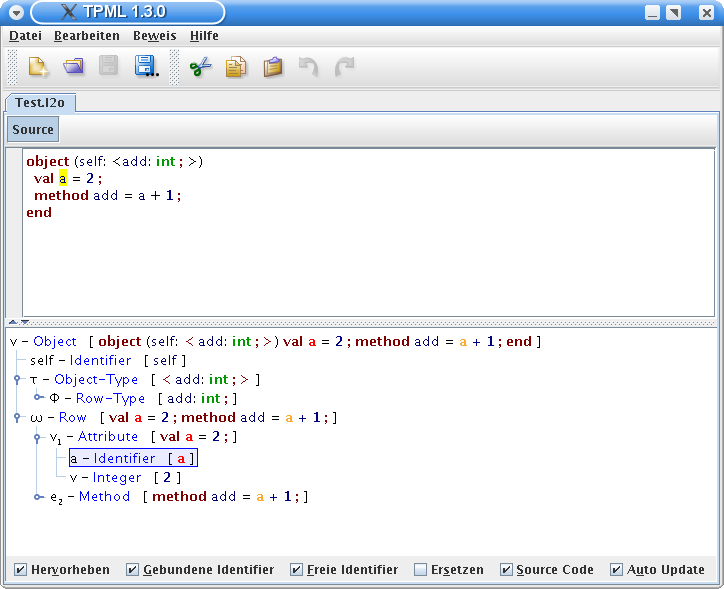
\includegraphics[width=10cm]{images/outline.png}
\caption{Outline}
\end{center}
\end{figure}

\subsection {Einstellungen}
Die Outline bietet verschiedene Einstellungsm"oglichenkeiten, die nun
kurz angesprochen werden sollen.

{\bf Hervorheben} bietet die M"oglichkeit, den aktuell in der Outline
selektierten Knoten in h"oheren Knoten zu markieren. Ist zum Beispiel
der Ausdruck \glqq$\bli{x}{\infix{+}{1}{1}}{x}$\grqq\ in der Outline geladen,
und der Knoten \glqq${\infix{+}{1}{1}}$\grqq\ selektiert, wird der zweite Ausdruck
in dem ersten hervorgehoben. Die Farbe der Hervorhebung kann, wie alle
anderen Farben auch, in den Einstellungen von \TPML\ ver"andert werden.

{\bf Gebundene} steht daf"ur, dass gebundene Identifier und Typ-Namen,
wenn sie in der Outline selektiert werden, in h"oheren Knoten 
hervorgehoben werden. Der Ausdruck \glqq$\abstr{x}{\infix{+}{x}{1}}$\grqq\ besteht
aus einen Identifier \glqq$x$\grqq\ und aus einem Kind-Ausdruck
\glqq$\infix{+}{x}{1}$\grqq. Selektiert man nun den Identifier, werden bei
aktiver Option alle Identifier hervorgehoben, die an diesen Identifier
gebunden sind. Dies funktioniert auch umgekehrt, wird also das
\glqq$x$\grqq\ im Ausdruck \glqq$\infix{+}{x}{1}$\grqq\ selektiert, wird der
Identifier hervorgehoben, an den dieser Identifier gebunden ist. Vor allem
bei komplizierteren Ausdr"ucken mit gleichen Identifiern wie 
\glqq$\bli{x}{1}{\infix{+}{x}{\bli{x}{2}{x}}}$\grqq\ k"onnen so die Bindungen
durch die Outline "uberpr"uft werden.

Wenn {\bf Freie} aktiv ist, werden freie Identifier und Typ-Namen in der
Outline hervorgehoben. Dies ist besonders n"utzlich, da freie Identifier
oder Typ-Namen meist auf eine fehlerhafte Eingabe zur"uckzuf"uhren sind.
Gibt der Anwender zum Beispiel \glqq$\bli{x}{a}{x}$\grqq\ ein, ist 
dies nat"urlich nicht falsch, aber der Type Checker w"urde den Ausdruck
nicht akzeptieren, da das \glqq$a$\grqq\ in dem Ausdruck frei 
vorkommend ist. Es werden allerdings nur Identifier und Typ-Namen
hervorgehoben, die in dem Wurzel Knoten frei vorkommend sind und nicht
alle, in den jeweiligen Knoten frei vorkommenden Identifier oder Typ-Namen.

Die Option {\bf Ersetzen} steht daf"ur, dass der selektierte Ausdruck
in h"oheren Knoten durch \glqq...\grqq\ ersetzt wird. Dadurch
werden h"ohere Knoten kompakter dargestellt, was bei gr"o"seren Ausdr"ucken
von Vorteil ist.

Ist die Option {\bf Source Code} aktiv, wird der Source Code im jeweiligen
Quelltexteditor hervorgehoben, der dem selektierten Knoten in der Outline
entspricht. Ist diese Option nicht aktiv, kann der Source Code durch einen
Doppelklick auf den Outline Knoten ebenfalls hervorgehoben werden. Diese
Option ist nur bei den Quelltexteditor verf"ugbar und nicht bei den
verschiedenen Beweiswerkzeugen.

{\bf Auto Update} steht daf"ur, dass die Outline automatisch geladen wird,
wenn sich etwas "andert, dies geschieht nach einer gewollten Verz"ogerung,
die n"otig ist, damit sich nicht zu viele "Anderungen ergeben. Diese Option
ist nur in Ansichten aktiv, in denen "Anderungen eindeutig sind, also in den
Quelltexteditoren und im Small Step Interpreter. In den anderen
Beweiswerkzeugen k"onnen bei einem Schritt mehrere Knoten erzeugt werden
und ein Laden der Outline w"are nicht eindeutig m"oglich.
Ist die Option nicht aktiv oder gar nicht verf"ugbar, kann der Anwender auf 
die entsprechenden Ausdr"ucke oder Typen klicken und diese werden dann geladen.
Gleiches gilt f"ur die Quelltexteditoren, klickt man mit der Maus auf den
Editor, wird der aktuelle Ausdruck oder Typ in die Outline geladen. Ist im
Quelltexteditor im Moment kein g"ultiger Ausdruck geladen, wird die Outline
rot umrandet.


\section {Beweiswerkzeuge}
\label{Beweiswerkzeuge} Wird ein Beweiswerkzeug gestartet, so wird
es zus"atzlich zum Quelltexteditor im Tab der Datei angezeigt. F"ur
jede Datei kann jeweils nur ein Small Step Interpreter, ein Big Step
Interpreter, ein Type Checker usw. aktiv sein. Diese k"onnen "uber die
entsprechende Schaltfl"achen angew"ahlt werden. Nat"urlich ergibt es keinen Sinn, Beweiswerkzeuge, die mit dem Typsystem zu tun haben, bei Dateien zu starten, die kein Typsystem haben, wie beispielsweise \LZERO. Wird ein
Beweiswerkzeug erneut gestartet, so ersetzt der neue Beweis ein ggf.
schon aktives Beweiswerkzeug des selben Typs. M"ochte man also zum
Beispiel einen Small Step Beweis neu starten oder f"ur einen leicht
ge"anderten Ausdruck erneut ausf"uhren, so kann dies "uber eine
erneute Anwahl der Small Step Funktion im Men"u {\bf Beweis}
geschehen. Dabei wird jedoch der aktive Small Step Interpreter durch
den neuen ersetzt.

Jedes Beweiswerkzeug verf"ugt "uber einen {\bf Beginner} und einen
{\bf Fortgeschrittener} Modus. Diese Modi unterscheiden sich in den
Regeln, zum Beweis des Ausdrucks zur Verf"ugung stehen und teilweise in der Ansicht des Beweiswerkzeuges. So werden beispielsweise beim Typ Checker im {\bf Beginner} Typen erst dann angezeigt, wenn der Typ bewiesen ist.

\subsection {Mouse-Over-Effekt}
Jeder der Beweismethoden hat f"ur den Benutzer eine weitere Komfort-Funktion eingebaut. Bei gr"o"seren Programmen, die bewiesen werden sollen, und insbesondere, wenn der gleiche Identifier doppelt benutzt wird verliert man schnell die "Ubersicht. Folgendes Beispiel soll dies verdeutlichen:

{\bf $\bli{x}{\abstr{x}{\app{x}{x}}}{\app{x}{x}}$}

Wie man leicht sieht ist der Identifier \glqq$x$\grqq\ doppelt verwendet. In noch gr"o"seren Beispielen w"are es nicht mehr einfach zu "uberschauen, an welches \glqq$x$\grqq\ welches gebunden ist. Um dies zu vereinfachen kann man einfach mit dem Mauszeiger "uber eins der \glqq$x$\grqq\ fahren, und die dazugeh"origen \glqq$x$\grqq\ werden farbig hervorgehoben. Zus"atzlich wird der Identifier, an den die anderen gebunden sind extra durch eine andere Farbe hervorgehoben\footnote{Die Farben, sowohl f"ur gebundenen als auch bindende Indentifier k"onnen "uber Einstellungen... im Men"u Bearbeiten eingestellt werden.}. Im gegebenen Beispiel w"urde das \glqq$x$\grqq\ nach dem \glqq$let$\grqq\ zusammen mit den letzten beiden \glqq$x$\grqq\ hervorgehoben, w"arend das \glqq$x$\grqq\ nach dem \glqq$lambda$\grqq\ zusammen mit den folgenden beiden \glqq$x$\grqq\ hervorgehoben w"urden.
Idetifier, die keine Bindungen haben, aber Bindungen haben k"onnten werden ebenfalls hervorgehoben. Anders Identifier, die gar keine Bindungen haben k"onnen, wie es bei Namen f"ur Methoden der Fall ist. Dazu sei ein letzte Beispiel zu diesem Thema gegeben:

{\bf object (self) method inc x y = x + 1 ; end}

Dieses Beispiel hat drei Identifier: inc, x und y. x verh"alt sich wie im oberen Beispiel. Es wird zusammen mit dem gebundenen x hervorgehoben. y dagegen hat zwar keinen weiteren gebundenen Identifier, k"onnte aber einen solchen haben. Er wird alleine hervorgehoben. inc letzlich wird nicht hervorgehoben. Es ist ein Methodenname und an den kann prinzipiell nichts gebunden sein.

\section {Tutorials}
Im folgenden wird anhand von einigen Beispielen in die
Funktionsweise der einzelnen Beweiswerkzeuge eingef"uhrt. Zun"achst
"offnen wir "uber {\bf Datei} $\rightarrow$ {\bf Neu...} einen
Editor. Wie gesagt ist jeder Editor fest mit einer Sprache
verkn"upft.

\begin{figure}[h]
\begin{center}
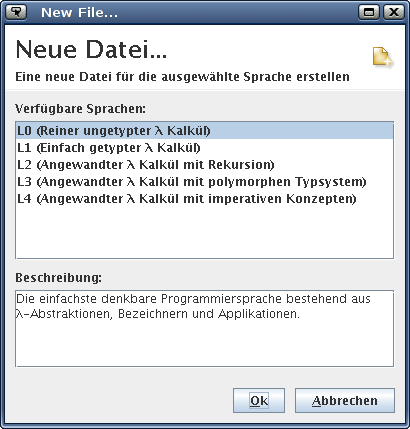
\includegraphics[width=8cm]{images/new-dialog.png}
\caption{Eine neue Datei erstellen}
\end{center}
\end{figure}

Wir w"ahlen f"ur unser Beispiel die Sprache \LONE\ aus und best"atigen
mit {\bf Ok}. Es ist nun standardm"a"sig der Quelltexteditor aktiv.
Wir geben einen Ausdruck ein, mit dem wir nun arbeiten wollen:

{\bf (lambda x.x * 3) 4}

Mit ein wenig Vorstellungskraft erkennt man, dass dieser Ausdruck
vorraussichtlich das Produkt aus 3 und 4 berechnet.


\subsection{Small Step Interpreter}
Unsere mutige Behauptung wollen wir nun nat"urlich durch einen
stichhaltigen Beweis untermauern. Wir starten also mittels {\bf
Beweis} $\rightarrow$ {\bf Small Step} oder mit der Taste F9 einen
Small Step Interpreter.

\begin{figure}[h]
\begin{center}
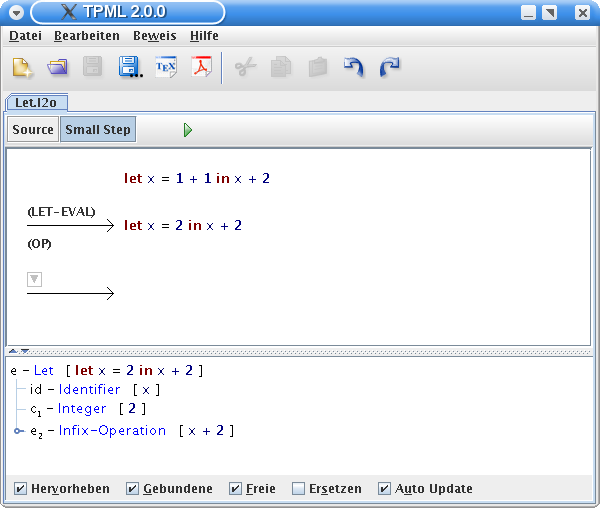
\includegraphics[width=10cm]{images/small-step.png}
\caption{Der Small Step Interpreter}
\label{FigureSmallStep}
\end{center}
\end{figure}

Bewegt man nun den Mauscursor "uber den Buttons des Regelmen"us
oberhalb des Pfeils f"ur den ersten Ableitungsschritt wird der Teil
des Ausdrucks rot unterstrichen, der als n"achstes Abgeleitet werden
soll, wie in Abbildung~\ref{FigureSmallStep} gezeigt.
In unserem Falle ist dies der gesamte Ausdruck. Der n"achste
Ableitungsschritt muss {\bf BETA-V} sein, um die 4 f"ur das x zu
substituieren. Wir klicken also auf den Button und w"ahlen in dem
erscheinenden Regelmen"u den entsprechenden Eintrag aus. Alternativ
kann man auch einzelne Schritte oder den kompletten Beweis
automatisch ausf"uhren lassen. F"ur einzelne Schritte klickt man
entweder auf den gr"unen Pfeil oberhalb des Small Step Interpreters
oder w"ahlt {\bf Raten} im Regelmen"u. Eine komplette Beweisf"uhrung
wird mittels {\bf Vervollst"andigen} im selben Men"u vorgenommen.

Ist man mit den Regeln vertraut, so kann man "uber {\bf Beweis}
$\rightarrow$ {\bf Fortgeschrittener} einige Regeln ausblenden. Das
Regelmen"u enth"alt nun nur noch Regeln die spezifizieren was getan
werden soll und nicht mehr genau wo. So muss zum Beispiel eine
Bedingung nicht mehr mit {\bf COND-EVAL} ausgewertet werden. Man
gibt w"ahlt lediglich {\bf COND-TRUE} bzw. {\bf COND-FALSE} aus.

\subsection{Big Step Interpreter}
Der Big Step Interpreter kann auch "uber das {\bf Beweis} Men"u oder
mit der Taste F11 gestartet werden. Zu beachten ist, dass man sich
hierf"ur nicht zwingend im Quelltexteditor befinden muss. Auch beim
Big Step Interpreter k"onnen Regeln "uber das Regelmen"u ausgew"ahlt
werden. Ist ein Unterbaum vollst"andig ausgewertet, so wird das
ermittelte Ergebnis f"ur h"ohere Knoten "ubernommen. Da unser
Beispiel lediglich einen Unterbaum f"ur die Regel {\bf BETA-VALUE}
enth"alt, ist dies auch gleichzeitig unser Ergebnis. Im Gegensatz
zum Small Step Interpreter gibt es aufgrund der Baumstruktur des
Beweises mehrere Stellen an denen Regeln angewandt werden k"onnen.
Die Raten-Funktion bezieht sich dabei immer auf den obersten, noch
nicht komplett ausgewerteten Teilbaum. Mit {\bf Vervollst"andigen}
wird stets nur der jeweilige Unterbaum komplett ausgewertet und
nicht wie beim Small Step Interpreter der komplette Beweis zu ende
gef"uhrt.

\subsection{Type Checker}

Diese Beweisart ist genau wie der Big Step Interpreter in einer
Baumstruktur aufgebaut. Der Type Checker verh"alt sich daher
bez"uglich des Anwenden von Regeln, den Raten und der
Vervollst"andigen Funktion genau wie der Big Step Interpreter. Das
Anf"ugen von Typvariablen geschieht bei Regelanwendung automatisch.

Alternativ kann man mit der Funktion {\bf Typ eingeben} in dem
Regelmen"u selbst einen Typ f"ur den entsprechenden Teilbaum
eingeben, wie in Abbildung~\ref{FigureTypeChecker} gezeigt.
Der Typinferenzalgorithmus versucht dann den Unterbaum zu
diesem Typ auszuwerten.

\begin{figure}[h]
\begin{center}
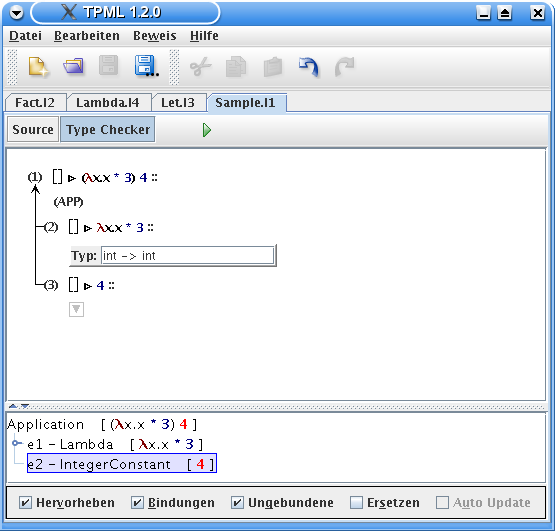
\includegraphics[width=10cm]{images/type-checker.png}
\caption{Der Type Checker}
\label{FigureTypeChecker}
\end{center}
\end{figure}

\subsection{Type Inference}
Der Type Inference Algorithmus ist, wie der Small Step Interpreter 
auch, in einer Listenstruktur realisiert, und kann "uber {\bf Beweis} 
$\rightarrow$ {\bf Type Inference} gestartet werden. Die Bedienung ist auch diesmal 
wieder an die bereits genannten Beweisarten angelehnt. Es besteht 
auch hier die M"oglichkeit selber Regeln auf den aktuellen Ausdruck
anzuwenden, den n"achsten Schritt erraten zu lassen, oder den kompletten
Ausdruck zu vervollst"andigen.

Wendet man die Regel Unify an, werden die evtl. daraus hervorgehenden
Type Substitutions in einer Liste "uber den Type Formulas gesammelt. 
Dabei ist die zuletzt gesammelte Type Substitution sichtbar. Die bereits
vorher gesammelten Type Substitutions werden durch drei Punkte angedeutet,
und k"onnen als Tooltip "uber den Punkten eingesehen werden.

Wenn man sich etwas mit der Funktionsweise des Algorithmus vertraut gemacht hat,
kann man "uber {\bf Beweis} $\rightarrow$ {\bf Fortgeschrittener} in den 
Advanced Modus wechseln. In diesem Modus werden Type Equations, bei denen beide
Typvariablen aus Arrow Types bestehen, jetzt nicht mehr neue Type Equations
aufgenommen, sondern diese werden direkt zu Type Substitutions aufgel"ost.
Ausserdem wird beim Anwenden einer Regel auf den Ausdruck nicht mehr vom System
versucht die Regel einer Type Formula zuzuordnen, sondern es wird versucht die Regel
auf die erste Type Formula anzuwenden. Diese k"onnen allerdings durch Drag 
and Drop umsortiert werden.

Das Regelwerk ist, mit einer Ausnahme, "aquivalent zum Type Checker. Es wurde 
noch die Regel {\bf UNIFY} hinzugenommen. Die sich aus folgenden Ableitungsschritten
zusammensetzt:\\[4mm] 

\begin{tabular}{ll}
  (EMPTY)\    & $\unify(A,\emp) = [\,]$ \\[3mm]
  (ASSUME)\   & $\unify(A,\{\tau = \tau'\} \cup E) = \unify(A,E) \mbox{  falls } (\tau = \tau') \in A $\\[3mm]
  (TRIV)\     & $\unify(A,\{\tau = \tau\} \cup E) = \unify(A,E)$\\[3mm]
  (MU-LEFT)\  & $\unify(A,\{\rectype{t}{\tau} = \tau'\} \cup E) = 
                 \unify(A,\{\tau [\rectype{t}{\tau}/t] = \tau'\} \cup E)$\\[3mm]
  (MU-RIGHT)\ & $\unify(A,\{\tau = \rectype{t}{\tau'}\} \cup E) = 
                 \unify(A,\{\tau = \tau' [\rectype{t}{\tau'}/t]\} \cup E)$\\[3mm]
  (VAR)\      & $\unify(A,\{\alpha = \tau\} \cup E) = \unify(A,\{\tau = \alpha\} \cup E)$\\[2mm]
              & $\ =\, \bcase 
                        [\tau/\alpha] \circ s & 
                        \mbox{falls } \alpha \notin \var{\tau} \mbox{ und } 
                        \unify(E[\tau/\alpha]) = s \\[2mm]
                        \fail         & \mbox{falls } \alpha \notin \var{\tau} \mbox{ und }\\&
                        \unify(E[\tau/\alpha]) = \fail\\[1mm]
                        & \mbox{oder } \alpha \in \var{\tau} \mbox{ und } \alpha \neq \tau
                        \ecase\vspace{3mm}$\\
  (ARROW)\    & $\unify(A,\{\tau_1 \to \tau_2 = \tau'_1 \to \tau'_2\} \cup E)$\\[1mm]
              & \quad $= \unify(A \cup \{\tau_1 \to \tau_2 = \tau'_1 \to \tau'_2\},
                \{\tau_1 = \tau'_1,\,\tau_2 = \tau'_2\} \cup E)$\\[3mm]
  (TUPLE)\    & $\unify(A,\{\tau_1 *\ \ldots\ * \tau_n = \tau_1' *\ \ldots\ * \tau_n'\} \cup E)$\\[1mm]
              & \quad $= \unify(A \cup \{\tau_1 *\ \ldots\ * \tau_n = \tau_1' *\ \ldots\ * \tau_n'\},$\\
              & \quad \quad $\{\tau_1 = \tau_1',\ \ldots\ , \tau_n = \tau_n'\} \cup E)$\\[3mm]
  (LIST)\     & $\unify(A,\{\listtype{\tau} = \listtype{\tau'} \} \cup E)$\\[1mm]
              & \quad $= \unify(A \cup \{\listtype{\tau} = \listtype{\tau'} \},
                         \{\tau = \tau' \} \cup E)$\\[3mm]
  (REF)\      & $\unify(A,\{\reftype{\tau} = \reftype{\tau'} \} \cup E)$\\[1mm]
              & \quad $= \unify(A \cup \{\reftype{\tau} = \reftype{\tau'} \},
                         \{\tau = \tau' \} \cup E)$\\[3mm]
  (OBJECT)\   & $\unify(A,\{\objecttype{\phi}\ =\ \objecttype{\phi'} \} \cup E)$\\[1mm]
              & \quad $= \unify(A \cup \{\objecttype{\phi}\ =\ \objecttype{\phi'} \},
                         \{\phi = \phi' \} \cup E)$\\[3mm]
  (ROW)\      & $\unify(A,\{ (m_1 = \tau_1\ ;\ \ldots\ ;\ m_n = \tau_n;\ \phi)$\\
              & \quad $= (m_1 = \tau_1'\ ;\ \ldots\ ;\ m_n = \tau_n';\ \phi') \} \cup E)$\\[1mm]
              & \quad $= \unify(A \cup \{ (m_1 = \tau_1\ ;\ \ldots\ ;\ m_n = \tau_n;\ \phi)$\\
              & \quad \quad $= (m_1 = \tau_1'\ ;\ \ldots\ ;\ m_n = \tau_n';\ \phi') \},$\\
              & \quad \quad \quad $\{\tau_1 = \tau_1', \ \ldots\ ,\tau_n = \tau_n',
                \phi = \phi' \} \cup E)$\\[3mm]
  (STRUCT)\   & $\unify(A,\{\tau_1 = \tau_2\} \cup E) = \fail$\\[1mm]
              & in  allen anderen F\"allen
\end{tabular}\\[6mm]
Bei der Regel {\bf ROW} ist darauf zu achten, dass die Methodennamen nicht in der gleichen Reihenfolge
vorkommen m"ussen. Ebenfalls m"ussen die Methodennamen nicht in beiden Reihen vorkommen, da f"ur den Fall, 
dass $\phi$ nicht gleich $\epsilon$ ist, $\unify$ auch mit $\phi$ und den restlichen Methoden von $\tau'$ 
aufgerufen werden kann. Zum Beispiel f"uhrt $\unify (A,\{ (b: \alpha_1 ; \alpha_2) = (a: int ; b: int ;)\}
\cup E)$ zu dem Aufruf von $\unify (A \cup \{ (b: \alpha_1 ; \alpha_2) = (a: int ; b: int ;)\},
\{\alpha_1 = int, \alpha_2 = a: int\} \cup E)$.

\subsection{Minimal Typing}
Der Minimal Typing Algorithmus ist, wie der Big Stepper und der Type Checker, in einer Baumstruktur realisiert.
Auch die Bedienung dieser Beweismethode ist "aquivalent zu den beiden anderen. Es besteht auch hier die M"oglichkeit
die n"achste Regel "uber das Pull Down Men"u auszuw"ahlen, einen Schritt vom Algorithmus selbst erraten zu lassen,
oder den kompletten Beweis vervollst"andigen zu lassen. F"ur den Fall, dass der Ausdruck synktaktischen Zucker 
enth"alt, kann auch hier in Kernsyntax "ubersetzt werden.

\subsection{Sub Typing}
Zur "Uberpr"ufung von Subtyprelationen wurde ein eigener Source Editor angelegt. Dieser beinhaltet zwei Eingabefelder,
welche von Bedienung und Aussehen dem normalen Source Editor gleichen, allerdings nur f"ur die Eingabe von Typen gedacht
sind, und nicht f"ur ganze Expressions. Das erste Eingabefeld soll den Subtyp entgegennehmen, und das zweite Eingabefeld 
den Supertyp, fu"r welche man die Subtyp Realation "uberpr"ufen will. Ein weiterer Unterschied zum allgemeinen Source 
Editor ist, dass man eine Outline pro Eingabefeld hat, statt wie vorher insgesamt eine Outline.

F"ur den Beweis hat man die Wahl zwischen einfachem Sub Typing, und Sub Typing mit rekursiven Typen. Beide sind von 
Bedienung und Aussehen her exakt gleich. Auch hier wurde bei der Visualisierung wieder eine Baumstruktur verwendet,
und von die Bedienung gleicht Subtyping den schon bekannten Beweismethoden. 



% vi:set syntax=tex ts=2 sw=2 et encoding=UTF-8:


%% Die Sprachen im Detail
%% $Id$
%%
%% Kapitel 3 - Die Sprachen im Detail
%%

\chapter{Die Sprachen im Detail\label{DieSprachenImDetail}}

Dieses Kapitel beschreibt die in \TPML\ verf"ugbaren Sprachen im Detail. Dies beinhaltet sowohl die abstrakte Syntax der Sprachen als auch die
operationelle Semantik und das Typsystem, also die Regeln f"ur die big und small step Interpreter und den Type Checker. Dieses Kapitel ist
jedoch nicht geeignet als Ersatz f"ur den Besuch der Vorlesung oder "Ubung, ebensowenig sollte dieses Handbuch als vollst"andiges Skript
mi"sverstanden werden\footnote{Es mag wiederum allerdings n"utzlich als Grundlage f"ur die Pr"ufungsvorbereitung sein, da es eine vollst"andige
Auflistung des Regelwerks darstellt, welches jedoch nicht hunderprozentig mit dem Vorlesungsinhalt "ubereinstimmt.}.

Die Sprachen \LZERO\ bis \LFOUR\ sind strikt hierarchisch aufgebaut, das hei"st die Sprache $\mathcal{L}_{n+1}$ erweitert die Sprache
$\mathcal{L}_n$ ($0 \le n < 4$), beinhaltet also alle Merkmale der Sprache $\mathcal{L}_n$. Die Sprachen entsprechen im wesentlichen
den in der Vorlesung behandelten Sprachen. Kleinere Abweichungen sind jedoch m"oglich und stellenweise nicht vermeidbar. In der "Ubung
werden, falls notwendig, diese Abweichungen herausgestellt und erl"autert.



\section{Die Sprache \LZERO}

Die Sprache \LZERO\ stellt die einfachste denkbare Programmiersprache dar und entspricht dem \Define{reinen ungetypten $\lambda$-Kalk"ul}{reiner
ungetypter $\lambda$-Kalk"ul} \engl{pure untyped $\lambda$-calculus}. Die abstrakte Syntax enth"alt lediglich drei Produktionen.
\bgram
e \is \id
  \al \abstr{id}{e}
  \al e_1\,e_2
\egram
Ein g"ultiger Ausdruck ist also entweder ein Bezeichner, eine \notation{$\lambda$-Abstraktion} oder eine \notation{Applikation}.
Die Menge \notation{$\Val$}\ $\sleq \Exp$ der \Define{Werte}{Wert} \Engl{values}{value} \notation{$\name v$} wird durch
\bgram
v \is \id
  \al \abstr{id}{e}
\egram
definiert.


\subsection{Big step Semantik von \LZERO}

Ein \define{big step} ist eine Formel der Gestalt $e \eval v$ mit $r \in Val$. Ein big step hei"st g"ultig f"ur \LZERO, wenn
er sich mit den Regeln\\[5mm]
  \begin{tabular}{ll}
     \mbox{(VAL)}         & $v \eval v$ \\[3mm]
     \mbox{(BETA-V)}      & $\regel{e[v/\id] \eval v'}
                                   {(\abstr{id}{e})\,v \eval v'}$ \\[5mm]
     \mbox{(APP)}         & $\regel{e_1 \eval v_1 \quad e_2 \eval v_2 \quad v_1\,v_2 \eval v}
                                   {e_1\,e_2 \eval v}$
  \end{tabular}\\[7mm]
herleiten l"asst.


\subsection{Small step Semantik von \LZERO}

Ein \define{small step} ist eine Formel der Gestalt $e \to e'$. Ein small step hei"st g"ultig f"ur \LZERO, wenn er sich mit den
Regeln\\[5mm]
   \begin{tabular}{ll}
     \mbox{(BETA-V)}      & $(\abstr{id}{e})\,v \to e[v/\id]$ \\[5mm]
     \mbox{(APP-LEFT)}    & $\regel{e_1\to e'_1}
                               {e_1\,e_2 \to e'_1\,e_2}$ \\[3mm]
     \mbox{(APP-RIGHT)\ } & $\regel{e \to e'}
                                  {v\,e \to v\,e'}$
\end{tabular}\\[7mm]
herleiten l"asst.



\section{Die Sprache \LZEROCBN}

\index{Call By Name}
Die Sprache \LZEROCBN \ bietet den gleichen Funktionsumfang wie die Sprache \LZERO, benutzt aber statt der 
Call by Value eine Call by Name Semantik. Um dies zu realisieren werden verschiedene Regeln in der Big step 
und der Small step Semantik gel"oscht oder ge"andert. Nur diese ge"anderten bzw. gel"oschten Regeln werden hier
aufgef"uhrt.

\subsection{Big step Semantik von \LZEROCBN}

Ein \notation{big step} hei"st g"ultig f"ur \LZEROCBN, wenn er sich mit den big step Regeln von \LZERO\ und den ge"anderten bzw. gel"oschten Regeln\\[5mm]
  \begin{tabular}{ll}
     \mbox{(BETA-V)}      & nicht vorhanden \\[3mm]
     \mbox{(BETA)}        & $\regel{e_1[e_2/\id] \eval v}
                                   {(\abstr{id}{e_1})\,e_2 \eval v}$ \\[5mm]
     \mbox{(APP)}         & nicht vorhanden \\[3mm]
     \mbox{(APP-LEFT)}    & $\regel{e_1 \eval v_1 \quad v_1\,e_2 \eval v}
                                   {e_1\,e_2 \eval v}$ \\[3mm]
     \mbox{(APP-RIGHT)}   & $\regel{e_2 \eval v_2 \quad v_1\,v_2 \eval v}
                                   {v_1\,e_2 \eval v}$   \ 
                                   falls ${v_1}$ nicht von der Form $\abstr{id}{e}$
  \end{tabular}\\[7mm]
herleiten l"asst.


\subsection{Small step Semantik von \LZEROCBN}

Ein \notation{small step} hei"st g"ultig f"ur \LZEROCBN, wenn er sich mit den small step Regeln von \LZERO\ 
und den ge"anderten bzw. gel"oschten Regeln\\[5mm]
  \begin{tabular}{ll}
     \mbox{(BETA-V)}      & nicht vorhanden \\[3mm]
     \mbox{(BETA)}        & $(\abstr{id}{e_1})\,e_2 \to e_1[e_2/\id]$ \\[5mm]
     \mbox{(APP-RIGHT)\ } & $\regel{e \to e'}
                                   {v\,e \to v\,e'}$   \ 
                                   falls ${v}$ nicht von der Form $\abstr{id}{e_0}$
  \end{tabular}\\[7mm]
herleiten l"asst.



\section{Die Sprache \LONE}

Die Sprache \LONE\ erweitert \LZERO\ um Konstanten, bedingte Ausf"uhrung, den Bindungsmechanismus $\blet$, Ausnahmen
\engl{exceptions} und ein einfaches Typsystem, entspricht damit also dem einfach getypten $\lambda$-Kalk"ul. Vorgegeben seien:
\bitem
  \item eine Menge $\Exn$ von \Define{Ausnahmen}{Ausnahme} $\exn$ \[\Exn = \{ divide\_by\_zero \}\]
  \item f"ur jeden arithmetischen Operator $\op$ eine Funktion \[\op^\I: \Int \times \Int \to \Int \cup \Exn\]
  \item f"ur jeden Vergleichsoperator $\op$ eine Funktion \[\op^\I: \Int \times \Int \to \Bool\]
\eitem
Die Menge \notation{$\Type$} der \Define{Typen}{Typ} \Engl{types}{type} $\tau$ ist definiert durch:
\bgram
  \tau \is \bool \mid \inttype \mid \unit
       \al \arrowtype{\tau_1}{\tau_2}
       \al \mu t.\tau
       \al t
\egram
Die abstrakte Syntax, definiert durch die Menge $\Exp$ der g"ultigen Ausdr"ucke, wird erweitert durch neue Produktionen
\bgram
e \is c
  \al \abstr{\id: \tau}{e}
  \al \bli{\id}{e_1}{e_2}
  \al \bli{\id: \tau}{e_1}{e_2}
  \al \bifte{e_0}{e_1}{e_2}
  \al e_1\,\op\,e_2
  \al \andalso{e_1}{e_2}
  \al \orelse{e_1}{e_2}
  \al \coercion{e}{\tau}{\tau'}
\egram
wobei die Menge \notation{$\Const$} der \Define{Konstanten}{Konstante} \Engl{constants}{constant} $c$ durch
\bgram
c \is \nop                    & & \mbox{unit-Element}
  \al b \in \{\true,\false\}  & & \mbox{boolescher Wert}
  \al n \in \setZ             & & \mbox{ganze Zahl} 
  \al \op                     & & \mbox{Operator} 
\egram
und die Menge \notation{$\Op$} der \Define{Operatoren}{Operator} \Engl{operators}{operator} $\op$ durch
\bgram
\op \is + \ \mid\  - \ \mid\  * \ \mid\ / \ \mid \ \mbox{mod}     & & \mbox{arithmetische Operatoren}
    \al < \ \ \mid\ \ > \ \ \mid\ \ \leq \ \ \mid\ \  \geq \ |\ = & & \mbox{Vergleichsoperatoren}
    \al \Not                                                & & \mbox{Negation}
\egram
definiert ist. Die Menge \notation{$\Val$} der Werte $v$ wird um die Produktionen
\bgram
v \is c
  \al \op\,e_1
  \al \abstr{\id: \tau}{e}
\egram
erweitert. F"ur Zahlkonstanten existiert derzeit die Einschr"ankung, dass nur positive Ziffernfolgen vom Lexer
akzeptiert werden. Negative Zahlen k"onnen aber bei Bedarf durch Subtraktion konstruiert werden ($0 - n$ f"ur
$n \in \setN$).

Die Angabe eines Typs bei $\lambda$-Abstraktion und $\blet$ ist also optional, und f"ur den big und small step
Interpreter werden die Typangaben einfach ignoriert. Der Typechecker bestimmt bei $\abstr{\id}{e}$ den Typ f"ur
$\id$ mittels Typinferenz, w"ahrend bei $\blet$ die Angabe des Typs lediglich als zus"atzliche Sicherheit f"ur
den Programmierer dient.


\subsection{Big step Semantik von \LONE}

Ein \notation{big step} hei"st g"ultig f"ur \LONE, wenn er sich mit den big step Regeln von \LZERO, den Regeln\\[5mm]
  \begin{tabular}{ll}
     \mbox{(AND-FALSE)}   & $\regel{e_1 \eval \false}
                                   {\andalso{e_1}{e_2} \eval \false}$ \\[5mm]
     \mbox{(AND-TRUE)}    & $\regel{e_1 \eval \true \quad e_2 \eval v}
                                   {\andalso{e_1}{e_2} \eval v}$ \\[5mm]
     \mbox{(COND-TRUE)}   & $\regel{e_0 \eval \true \quad e_1 \eval v}
                                   {\bifte{e_0}{e_1}{e_2} \eval v}$ \\[5mm]
     \mbox{(COND-FALSE)}  & $\regel{e_0 \eval \false \quad e_2 \eval v}
                                   {\bifte{e_0}{e_1}{e_2} \eval v}$ \\[5mm]
     \mbox{(LET)}         & $\regel{e_1 \eval v_1 \quad e_2[v_1/\id] \eval v_2}
                                   {\bli{\id}{e_1}{e_2} \eval v_2}$ \\[5mm]
     \mbox{(NOT)}         & $\Not\,b \eval \neg b$ \\[3mm]
     \mbox{(OP)}          & $\op\,n_1\,n_2 \eval \op^{\I}(n_1,n_2)$ \\[3mm]
     \mbox{(OR-FALSE)}    & $\regel{e_1 \eval \false\quad e_2 \eval v}
                                   {\orelse{e_1}{e_2} \eval v}$ \\[5mm]
     \mbox{(OR-TRUE)}     & $\regel{e_1 \eval \true}
                                   {\orelse{e_1}{e_2} \eval \true}$\\[5mm]
     \mbox{(COERCE)}      & $\regel{e \eval v}
                                   {\coercion{e}{\tau}{\tau'} \eval v}$
  \end{tabular}\\[7mm]
und mit den zugeh"origen exception-Regeln herleiten l"asst. Diese exception-Regeln erh"alt man
aus den obigen Regeln indem man zu jeder Regel der Form\\[2mm]
   \begin{tabular}{ll}
     \mbox{(R)} & $\regel{e_1 \eval v_1 \quad \ldots \quad  e_n \eval v_n}
                         {e \eval v}$

   \end{tabular}\\[3mm]
(d.h.\ zu jeder Regel mit $n$ Pr\"amissen) f\"ur jedes $1 \le i \le n$ die Regel \\[3mm]
   \begin{tabular}{ll}
      \mbox{(R-EXN-$i$)} & $\regel{e_1 \eval v_1 \quad \ldots \quad e_{i-1} \eval v_{i-1} \quad e_i \eval \exn}
                                {e \eval \exn}$ \\[5mm]
   \end{tabular}\\[3mm]
hinzuf"ugt. Exception-Regeln m"ussen beim big step Interpreter nicht explizit ausgew"ahlt werden, sonde\mbox werden
automatisch eingesetzt, sobald eine Ausnahme weitergereicht werden mu"s.


\subsection{Small step Semantik von \LONE}

Ein \notation{small step} hei"st g"ultig f"ur \LONE, wenn er sich mit den small step Regeln von \LZERO, den Regeln\\[5mm]
  \begin{tabular}{ll}
    \mbox{(AND-EVAL)}     & $\regel{e_1 \to e_1'}
                                 {\andalso{e_1}{e_2} \to \andalso{e_1'}{e_2}}$\\[5mm]
    \mbox{(AND-FALSE)}    & $\andalso{\false}{e_2} \to \false$\\[3mm]
    \mbox{(AND-TRUE)}     & $\andalso{\true}{e_2} \to e_2$\\[3mm]
    \mbox{(NOT)}          & $\Not\,b \to \neg b$\\[3mm]
    \mbox{(OP)}           & $\op\,n_1\,n_2 \to \op^{\I}(n_1,n_2)$ \\[3mm]
    \mbox{(COND-EVAL)\ }  & $\regel{e_0 \to e'_0}
                            {\bifte{e_0}{e_1}{e_2} \to \bifte{e'_0}{e_1}{e_2}}$ \\[5mm]
    \mbox{(COND-TRUE)\ }  & $\bifte{\true}{e_1}{e_2} \to e_1$ \\[3mm]
    \mbox{(COND-FALSE) }  & $\bifte{\false}{e_1}{e_2} \to e_2$ \\[3mm]
    \mbox{(LET-EVAL)\  }  & $\regel{e_1 \to e'_1}
                            {\bli{\id}{e_1}{e_2} \to \bli{\id}{e'_1}{e_2}}$ \\[5mm]
    \mbox{(LET-EXEC)}       & $\bli{\id}{v}{e} \to e[v/\id]$ \\[5mm]
    \mbox{(OR-EVAL)}      & $\regel{e_1 \to e_1'}
                                   {\orelse{e_1}{e_2} \to \orelse{e_1'}{e_2}}$\\[5mm]
    \mbox{(OR-FALSE)}     & $\orelse{\false}{e_2} \to e_2$\\[3mm]
    \mbox{(OR-TRUE)}      & $\orelse{\true}{e_2} \to \true$\\[3mm]
    \mbox{(COERCE)}       & $\coercion{e}{\tau}{\tau'} \to e$
  \end{tabular}\\[7mm]
und mit den zugeh"origen exception-Regeln herleiten l"asst. Diese exceptions-Regeln erh"alt man - "ahnlich wie
bei der big step Seminatik - aus den obigen Regeln indem man f"ur jede Regel der Form\\[2mm]
  \begin{tabular}{ll}
    \mbox{(R)} & $\regel{e_1 \to e'_1}{e_2 \to e'_2}$
  \end{tabular}\\[3mm]
(d.h.\ zu jeder Regel mit Pr\"amisse) die Regel \\[3mm]
  \begin{tabular}{ll}
    \mbox{(R-EXN)} & $\regel{e_1 \to \exn}{e_2 \to \exn}$
  \end{tabular}\\[3mm]
hinzunimmt. Wie beim big step Interpreter gilt auch f"ur den small step Interpreter, dass exception-Regeln nicht
explizit angegeben werden m"ussen.


\subsection{Typechecker Semantik von \LONE}

\LONE\ verf"ugt "uber ein einfaches \notation{Typsystem}, benutzt aber wie alle folgenden Sprachen schon den
\notation{Typinferenzalgorithmus}, was anfangs vielleicht zu schwer verst"andlichen Fehlermeldungen f"uhren kann.
In diesem Fall sollte es in der "Ubung angesprochen werden.

Ein \define{Typurteil} f"ur Ausdr"ucke ist von der Form $\Tj{\Gamma}{e}{\tau}$, wobei $\Gamma: \Id \pto \Type$ eine
partielle Funktion mit endlichem Definitionsbereich ist, die bestimmten Bezeichne\mbox einen Typ zuordnet. $\Gamma$ wird
als \define{Typumgebung} \engl{type environment} bezeichnet. Ein Typurteil heisst g"ultig f"ur \LONE, wenn es sich mit
den Regeln\\[3mm]
\begin{tabular}{ll}
  \mbox{(CONST)\  } & $\regel{\tj{c}{\tau}}
                           {\Tj{\Gamma}{c}{\tau}}$\\[5mm]
  \mbox{(ID)\     } & $\Tj{\Gamma}{\id}{\tau}$ \reason{falls $\id \in \dom \Gamma$ und $\Gamma(\id) = \tau$}\\[5mm]
  \mbox{(APP)\    } & $\regel{\Tj{\Gamma}{e_1}{\tau\to\tau'} 
                            \quad
                            \Tj{\Gamma}{e_2}{\tau}}
                           {\Tj{\Gamma}{e_1\,e_2}{\tau'}}$\\[5mm]
  \mbox{(COND)\   } & $\regel{\Tj{\Gamma}{e_0}{\bool}
                            \quad
                            \Tj{\Gamma}{e_1}{\tau}
                            \quad
                            \Tj{\Gamma}{e_2}{\tau}}
                          {\Tj{\Gamma}{\bifte{e_0}{e_1}{e_2}}{\tau}}$\\[5mm]
  \mbox{(LET)\ } & $\regel{\Tj{\Gamma}{e_1}{\tau_1}
                            \quad
                            \Tj{\Gamma[\tau_1/\id]}{e_2}{\tau_2}}
                           {\Tj{\Gamma}{\bli{\id}{e_1}{e_2}}{\tau_2}}$\\[5mm]
  \mbox{(ABSTR)\  } & $\regel{\Tj{\Gamma[\tau/\id]}{e}{\tau'}} 
                           {\Tj{\Gamma}{\abstr{\id:\tau}{e}}{\tau\to\tau'}}$ \\[5mm]
  \mbox{(AND)\ } & $\regel{\Tj{\Gamma}{e_1}{\bool} \quad \Tj{\Gamma}{e_2}{\bool}}
                          {\Tj{\Gamma}{\andalso{e_1}{e_2}}{\bool}}$ \\[5mm]
  \mbox{(OR)\  } & $\regel{\Tj{\Gamma}{e_1}{\bool} \quad \Tj{\Gamma}{e_2}{\bool}}
                          {\Tj{\Gamma}{\orelse{e_1}{e_2}}{\bool}}$\\[5mm]
  \mbox{(COERCE)\  } & $\regel{\Tj{\Gamma}{e}{\tau} \quad \subtype{\tau}{\tau'}}
                          {\Tj{\Gamma}{\coercion{e}{\tau}{\tau'}}{\tau'}}$
\end{tabular}\\[7mm]
herleiten l"asst. Die Regel (CONST) besagt hierbei, dass $c$ in der Typumgebung $\Gamma$ den Typ $\tau$ hat, wenn $c$
den Typ $\tau$ hat. Dies wird durch die Regeln\\[3mm]
\begin{tabular}{ll}
\mbox{(UNIT)\  } & $\tj{()}{\unit}$\\[2mm]
\mbox{(BOOL)\  } & $\tj{b}{\bool}$\\[2mm]
\mbox{(INT)\   } & $\tj{n}{\inttype}$\\[2mm]
\mbox{(NOT)\   } & $\tj{\Not}{\bool\to\bool}$\\[2mm]
\mbox{(AOP)\   } & $\tj{\op}{\inttype\to\inttype\to\inttype}$ 
                    \reason{ falls $\op$ arithmetischer Operator}\\[2mm]
\mbox{(ROP)\   } & $\tj{\op}{\inttype\to\inttype\to\bool}$ \reason{ falls $\op$ Vergleichsoperator}
\end{tabular}\\[7mm]
definiert. Beim Type Checker werden diese Regeln f"ur Konstanten nicht angegeben, sonde\mbox lediglich die (CONST) Regel.


\subsection{Minimal Typing Semantik von \LONE}

  Ein Typurteil $\Tjm{\Gamma}{e}{\tau}$ oder $\Tjm{\Gamma}{r}{\phi}$ heisst g\"ultig f\"ur \Lom,
  wenn es sich mit den Typregeln  \\[5mm]
  \begin{tabular}{ll} 
    \mbox{(Id)\ }           & $\Tjm{\Gamma}{\id}{\tau} \quad \text{falls } \id\in\dom{\Gamma} \wedge \Gamma(\id) = \tau$ \\[1mm]
    \mbox{(Const)\ }        & $\RULE{\tj{c}{\tau}}
                              {\Tjm{\Gamma}{c}{\tau}}$ \\[4mm]
    \mbox{(App-Subsume)\ }  & $\RULE{\Tjm{\Gamma}{e_1}{\typeArrow{\tau_2'}{\tau}}
                               \quad
                               \Tj{\Gamma}{e_2}{\tau_2}
                               \quad
                               \subtype{\tau_2} {\tau_2'}}
                              {\Tjm{\Gamma}{\expApp{e_1}{e_2}}{\tau}}$ \\[4mm]
    \mbox{(Abstr)\ }        & $\RULE{\Tjm{\Gamma\SUB{\tau}{x}}{e}{\tau'}}
                              {\Tjm{\Gamma}{\expAbstr{x:\tau}{e}}{\typeArrow{\tau}{\tau'}}}$ \\[4mm]
    \mbox{(Let)\ }          & $\RULE{\Tjm{\Gamma}{e_1}{\tau_1}
                               \quad
                               \Tjm{\Gamma\SUB{\tau_1}{x}}{e_2}{\tau_2}}
                              {\Tjm{\Gamma}{\expLet{x}{e_1}{e_2}}{\tau_2}}$ \\[4mm]
   \mbox{(Cond-Subsume)\ } & $\RULE{\Tjm{\Gamma}{e_0}{\bool}
                               \quad
                               \Tjm{\Gamma}{e_1}{\tau_1}
                               \quad
                               \Tjm{\Gamma}{e_2}{\tau_2}}
                              {\Tjm{\Gamma}{\expCond{e_0}{e_1}{e_2}}{\tau_1 \vee \tau_2}}$ \\[4mm]
  \mbox{(AND)\ } & $\regel{\Tjm{\Gamma}{e_1}{\bool} \quad \Tjm{\Gamma}{e_2}{\bool}}
                          {\Tjm{\Gamma}{\andalso{e_1}{e_2}}{\bool}}$ \\[4mm]
  \mbox{(OR)\  } & $\regel{\Tjm{\Gamma}{e_1}{\bool} \quad \Tjm{\Gamma}{e_2}{\bool}}
                          {\Tjm{\Gamma}{\orelse{e_1}{e_2}}{\bool}}$\\[4mm]
   \mbox{(COERCE)\ } & $\regel{\Tj{\Gamma}{e}{\tau} \quad \subtype{\tau}{\tau'}} 
                          {\Tj{\Gamma}{\coercion{e}{\tau}{\tau'}}{\tau'}}$
   
  \end{tabular} \\[7mm]
  und den Suptyping Regeln herleiten l\"a"st.



\subsection{Syntaktischer Zucker}

Die Sprache \LONE\ und alle folgenden Sprachen enthalten \Define{syntaktischen Zucker}{syntaktischer Zucker} um das Schreiben
von Programmen zu vereinfachen. Der syntaktische Zucker l"asst sich dann anschlie"send in Kernsyntax "ubersetzen oder direkt
verarbeiten. Hierbei wurden aus Gr"unden der "Ubersichtlichkeit nicht immer abgeleitete Regeln f"ur den syntaktischen Zucker eingef"uhrt,
sonde\mbox es wird implizit eine Konvertierung des betreffenden Teilausdrucks in \notation{Kernsyntax} vorgenommen. F"ur \LONE\ betrifft dies
Ausdr"ucke, die Operatoren in \notation{Infixschreibweise} enthalten, und die logischen Operatoren $\mathbin{\&\&}$ und $\mathbin{||}$. Es gilt:
\beqns
e_1\,\op\,e_2\quad \mbox{steht f"ur}\quad (\op\,e_1)\,e_2
\eeqns
Beim small step Interpreter w"urden also die Regeln (APP-LEFT) und (OP) angewendet. Beim Schreiben von Programmen ist dar"uber
hinaus zu beachten, dass Operatoren, sofe\mbox sie nicht in Infixausdr"ucken auftauchen, immer geklammert werden m"ussen. Die
Funktion, die $1$ zu ihrem Parameter addiert wird also als
\[(+)\,1\]
geschrieben. Dies entspricht der OCaml-Konvention und ist notwendig, da der Parser sonst bei bestimmten Ausdr"ucken nicht
entscheiden kann, ob es ein Infixausdruck ist, oder der Operator als Parameter in eine Funktion eingesetzt werden soll. Zum
Beispiel l"asst sich
\[x + y\]
interpretieren als Infixaddition von $x$ und $y$ oder als Anwendung der Funktion $x$ auf die Parameter $+$ und $y$. Intuitiv
w"urde ein Mensch ersteres vermuten, der Parser f"ur die konkrete Syntax kann dies jedoch nicht entscheiden.

Die logischen $\mathbin{\&\&}$- und 
$\mathbin{||}$-Verkn"upfungen sind syntaktischer Zucker f"ur die bedingte Ausf"uhrung
\beqns
  \andalso{e_1}{e_2} & \mbox{ steht f"ur } & \bifte{e_1}{e_2}{\false} \\
  \orelse{e_1}{e_2} & \mbox{ steht f"ur } & \bifte{e_1}{\true}{e_2}
\eeqns
und es existieren abgeleitete Interpreter- und Typregeln, da sonst der Umgang mit diesen Konstrukten zu aufwendig
w"are.

Interessant zu beobachten ist, dass auch der $\Not$-Operator als syntaktischer Zucker aufgefasst werden k"onnte.
\beqns
  \Not & \mbox{ steht f"ur } & \abstr{\id: \bool}{\bifte{\id}{\false}{\true}}
\eeqns
Dies sei aber nur am Rande erw"ahnt.



\section{Die Sprache \LONECBN}

\index{Call By Name}
Die Sprache \LONECBN \ bietet den gleichen Funktionsumfang wie die Sprache \LONE, benutzt aber statt der 
Call by Value eine Call by Name Semantik. Um dies zu realisieren werden verschiedene Regeln in der Big step 
und der Small step Semantik gel"oscht oder ge"andert. Nur diese ge"anderten bzw. gel"oschten Regeln werden hier
aufgef"uhrt.

\subsection{Big step Semantik von \LONECBN}

Ein \notation{big step} hei"st g"ultig f"ur \LONECBN, wenn er sich mit den big step Regeln von \LONE\ und den ge"anderten bzw. gel"oschten Regeln\\[5mm]
  \begin{tabular}{ll}
     \mbox{(BETA-V)}      & nicht vorhanden \\[3mm]
     \mbox{(BETA)}        & $\regel{e_1[e_2/\id] \eval v}
                                   {(\abstr{id}{e_1})\,e_2 \eval v}$ \\[5mm]
     \mbox{(APP)}         & nicht vorhanden \\[3mm]
     \mbox{(APP-LEFT)}    & $\regel{e_1 \eval v_1 \quad v_1\,e_2 \eval v}
                                   {e_1\,e_2 \eval v}$ \\[3mm]
     \mbox{(APP-RIGHT)}   & $\regel{e_2 \eval v_2 \quad v_1\,v_2 \eval v}
                                   {v_1\,e_2 \eval v}$   \ 
                                   falls ${v_1}$ nicht von der Form $\abstr{id}{e}$ \\[5mm]
     \mbox{(LET)}         & $\regel{e_2[e_1/\id] \eval v}
                                   {\bli{\id}{e_1}{e_2} \eval v}$
  \end{tabular}\\[7mm]
herleiten l"asst.


\subsection{Small step Semantik von \LONECBN}

Ein \notation{small step} hei"st g"ultig f"ur \LONECBN, wenn er sich mit den small step Regeln von \LONE\ 
und den ge"anderten bzw. gel"oschten Regeln\\[5mm]
  \begin{tabular}{ll}
     \mbox{(BETA-V)}      & nicht vorhanden \\[3mm]
     \mbox{(BETA)}        & $(\abstr{id}{e_1})\,e_2 \to e_1[e_2/\id]$ \\[5mm]
     \mbox{(APP-RIGHT)\ } & $\regel{e \to e'}
                                   {v\,e \to v\,e'}$   \ 
                                   falls ${v}$ nicht von der Form $\abstr{id}{e_0}$ \\[5mm]
     \mbox{(LET-EVAL)\  } & nicht vorhanden \\[3mm]
     \mbox{(LET-EXEC)}    & $\bli{\id}{e_1}{e_2} \to e_2[e_1/\id]$
  \end{tabular}\\[7mm]
herleiten l"asst.

\section{Die Sprache \LONESUB}
Die Sprache \LONESUB beschr"ankt sich auf das Typsystem von \LONE. 

\subsection{Sub Typing Semantik von \LONESUB}

Ein Beweisschritt f"ur Sub Typing hei"st g"ultig, wenn er sich mit den Regeln  \\[5mm]
  \begin{tabular}{ll}
    \mbox{(S-Refl)\ }       & $\subtype{\tau}{\tau}$  \\[1mm]
    \mbox{(S-Arrow)\ }      & $\RULE{\subtype{\tau_1'} {\tau_1} \quad \subtype {\tau_2} {\tau_2'}}
                              {\subtype{\typeArrow{\tau_1}{\tau_2}} {\typeArrow{\tau_1'}{\tau_2'}}}$ \\[4mm]
  \end{tabular} \\[7mm]

herleiten l\"a"st.

\subsection{Rec Sub Typing Semantik von \LONESUB}

Ein Beweisschritt f"ur Rec Sub Typing hei"st g"ultig, wenn er sich mit den Regeln  \\[5mm]
 \begin{tabular}{lll}
            \mbox{(S-Refl)\ } & $A \vdash \subtype{\tau}{\tau}$ \\[1mm]
            \mbox{(S-Assume)\ } & $\RULE{(\subtype{\tau_1} {\tau_2)} \in A}
                                   {A \vdash \subtype{\tau_1} {\tau_2}}$ \\[2mm]
            \mbox{(S-Arrow)\ } & $\RULE{A' \vdash \subtype{\tau_1} {\tau_1'}
                                   \quad
                                   A' \vdash \subtype{\tau_2} {\tau_2'}}
                                  {A \vdash \subtype{\typeArrow{\tau_1}{\tau_2}}
                                   {\typeArrow{\tau_1'}{\tau_2'}}}$ 
                                  & mit $A' = A \cup \{\subtype{\typeArrow{\tau_1}{\tau_2}}
                                   {\typeArrow{\tau_1'}{\tau_2'}}\}$ \\[2mm]
            \mbox{(S-Mu-Left)\ } & $\RULE{A' \vdash \subtype{\tau_1\SUB{\typeRec{t}{\tau_1}}{t}}
                                     {\tau_2}}
                                    {A \vdash \subtype{\typeRec{t}{\tau_1}} {\tau_2}}$
                                   & mit $A' = A \cup \{\subtype{\typeRec{t}{\tau_1}} {\tau_2\}}$ \\[2mm]
            \mbox{(S-Mu-Right)\ } & $\RULE{A' \vdash \subtype{\tau_1}
                                     {\tau_2\SUB{\typeRec{t}{\tau_2}}{t}}}
                                    {A \vdash \subtype{\tau_1} {\typeRec{t}{\tau_2}}}$
                                   & mit $A' = A \cup \{\subtype{\tau_1} {\typeRec{t}{\tau_2}\}}$ \\[2mm]
          \end{tabular}


herleiten l\"a"st.



\section{Die Sprache \LTWO}

\index{Rekursion}
Die Sprache \LTWO\ erweitert \LONE\ um rekursive Ausdr"ucke\footnote{Wohlgemerkt aber nicht um rekursive Typen. Das
Typsystem schr"ankt die Sprache also st"arker ein, als dies bei \LONE\ der Fall ist.} und syntaktischen Zucker, der
es erlaubt Funktionen einfacher zu definieren, "ahnlich zu OCaml.

Die Menge \notation{$\Exp$} der g"ultigen Ausdr"ucke wird um die Produktionen
\bgram
e \is \rec{\id: \tau}{e}
  \al \bli{\id (\id_1: \tau_1)\ldots(\id_n: \tau_n):\tau}{e_1}{e_2}
  \al \bli{\brec\,\id (\id_1: \tau_1)\ldots(\id_n: \tau_n):\tau}{e_1}{e_2}
\egram
erweitert, wobei s"amtliche Typangaben optional sind. Bei $\blet$ und $\blet\,\brec$ m"ussen die Bezeichner f"ur die
Parameter nur dann geklammert werden, wenn ein Typ f"ur diesen Parameter angegeben wird.


\subsection{Big step Semantik von \LTWO}

Ein \notation{big step} hei"st g"ultig f"ur \LTWO, wenn er sich mit den big step Regeln von \LONE\ und der Regel\\[3mm]
  \begin{tabular}{ll}
    \mbox{(UNFOLD)}      & $\regel{e[\rec{\id}{e}/\id] \eval v}
                                  {\rec{\id}{e} \eval v}$
  \end{tabular}\\[7mm]
sowie der dazugeh"origen exception-Regel herleiten l"asst.


\subsection{Small step Semantik von \LTWO}

Ein \notation{small step} hei"st g"ultig f"ur \LTWO, wenn er sich mit den small step Regeln von \LONE\ und der Regel\\[3mm]
  \begin{tabular}{ll}
    \mbox{(UNFOLD)}     & $\rec{\id}{e} \to e[\rec{\id}{e}/\id]$
  \end{tabular}\\[7mm]
herleiten l"asst.


\subsection{Typechecker Semantik von \LTWO}

Ein \notation{Typurteil} hei"st g"ultig f"ur \LTWO, wenn es sich mit den Typregeln von \LONE\ und der Regel\\[3mm]
\begin{tabular}{ll}
\mbox{(REC)\ } & $\regel{\Tj{\Gamma[\tau/\id]}{e}{\tau}} 
                         {\Tj{\Gamma}{\rec{\id:\tau}{e}}{\tau}}$
\end{tabular}\\[7mm]
herleiten l"asst. Fehlt die Angabe des Typs $\tau$ bei $\brec$ wird der Typ f"ur $e$ durch den Typinferenzalgorithmus
bestimmt.

\subsection{Minimal Typing Semantik von \LTWO}

  Ein Typurteil $\Tjm{\Gamma}{e}{\tau}$ oder $\Tjm{\Gamma}{r}{\phi}$ heisst g\"ultig f\"ur \Lom,
  wenn es sich mit den Typregeln \\[5mm]
  \begin{tabular}{ll} 
    \mbox{(Rec-Subsume)\ }  & $\RULE{\Tjm{\Gamma\SUB{\tau}{x}}{e}{\tau'} \quad \tau' \le \tau}
                              {\Tjm{\Gamma}{\expRec{x:\tau}{e}}{\tau}}$ \\[4mm]
  \end{tabular} \\[7mm]
  und den Suptyping Regeln herleiten l\"a"st.


\subsection{Syntaktischer Zucker}

Die Sprache \LTWO\ enth"alt weitere Abk"urzungen zu den in \LONE\ definierten. Die folgenden Abk"urzungen stehen f"ur
die leichtere Definition von Funktionen zur Verf"ugung.
\beqns
  \bli{\id (\id_1: \tau_1)\ldots(\id_n: \tau_n):\tau}{e_1}{e_2}
\eeqns
steht f"ur
\beqns
  \bli{\id: \tau}{\abstr{\id_1: \tau_1}{\ldots\abstr{\id_n: \tau_n}{e_1}}}{e_2}
\eeqns
und
\beqns
  \bli{\brec\,\id (\id_1: \tau_1)\ldots(\id_n: \tau_n):\tau}{e_1}{e_2}
\eeqns
steht f"ur
\beqns
  \bli{\id: \tau}{\rec{\id: \tau}{\abstr{\id_1: \tau_1}{\ldots\abstr{\id_n: \tau_n}{e_1}}}}{e_2}\mbox{.}
\eeqns
F"ur diesen syntaktischen Zucker wurden keine abgeleiteten Regeln eingef"uhrt, stattdessen wird implizit
eine "Ubersetzung in \notation{Kernsyntax} vorgenommen.



\section{Die Sprache \LTWOCBN}

\index{Call By Name}
Die Sprache \LTWOCBN \ bietet den gleichen Funktionsumfang wie die Sprache \LTWO, benutzt aber statt der 
Call by Value eine Call by Name Semantik. Um dies zu realisieren werden verschiedene Regeln in der Big step 
und der Small step Semantik gel"oscht oder ge"andert. Nur diese ge"anderten bzw. gel"oschten Regeln werden hier
aufgef"uhrt.

\subsection{Big step Semantik von \LTWOCBN}

Ein \notation{big step} hei"st g"ultig f"ur \LTWOCBN, wenn er sich mit den big step Regeln von \LTWO\ und den ge"anderten bzw. gel"oschten Regeln\\[5mm]
  \begin{tabular}{ll}
     \mbox{(BETA-V)}      & nicht vorhanden \\[3mm]
     \mbox{(BETA)}        & $\regel{e_1[e_2/\id] \eval v}
                                   {(\abstr{id}{e_1})\,e_2 \eval v}$ \\[5mm]
     \mbox{(APP)}         & nicht vorhanden \\[3mm]
     \mbox{(APP-LEFT)}    & $\regel{e_1 \eval v_1 \quad v_1\,e_2 \eval v}
                                   {e_1\,e_2 \eval v}$ \\[3mm]
     \mbox{(APP-RIGHT)}   & $\regel{e_2 \eval v_2 \quad v_1\,v_2 \eval v}
                                   {v_1\,e_2 \eval v}$   \ 
                                   falls ${v_1}$ nicht von der Form $\abstr{id}{e}$ \\[5mm]
     \mbox{(LET)}         & $\regel{e_2[e_1/\id] \eval v}
                                   {\bli{\id}{e_1}{e_2} \eval v}$
  \end{tabular}\\[7mm]
herleiten l"asst.


\subsection{Small step Semantik von \LTWOCBN}

Ein \notation{small step} hei"st g"ultig f"ur \LTWOCBN, wenn er sich mit den small step Regeln von \LTWO\ 
und den ge"anderten bzw. gel"oschten Regeln\\[5mm]
  \begin{tabular}{ll}
     \mbox{(BETA-V)}      & nicht vorhanden \\[3mm]
     \mbox{(BETA)}        & $(\abstr{id}{e_1})\,e_2 \to e_1[e_2/\id]$ \\[5mm]
     \mbox{(APP-RIGHT)\ } & $\regel{e \to e'}
                                   {v\,e \to v\,e'}$   \ 
                                   falls ${v}$ nicht von der Form $\abstr{id}{e_0}$ \\[5mm]
     \mbox{(LET-EVAL)\  } & nicht vorhanden \\[3mm]
     \mbox{(LET-EXEC)}    & $\bli{\id}{e_1}{e_2} \to e_2[e_1/\id]$
  \end{tabular}\\[7mm]
herleiten l"asst.

\section{Die Sprache \LTWOSUB}
Die Sprache \LTWOSUB ist erweitert die Sprache \LONE um das Typsystem der Sprache \LTWO. 

\section{Die Sprache \LTWOO}
\index{Objekte}
Die Sprache \LTWOO \ erweitert die Sprache \LTWO\ um Objekte. Die Menge \notation{$\Exp$} der
g"ultigen Ausdr"ucke wird hierf"ur um die Produktionen
\bgram
e \is (\send{e}{m})                                                 & & \mbox{Methodenaufruf}
  \al \object {self: \tau}{r}                                       & & \mbox{Objekt}
  \al \duplication{a_1 = e_1;\ \ldots\ ;a_n = e_n}                  & & \mbox{Duplikation}
\egram
erweitert.
Die Menge \notation{$\Row$} aller \name{Reihen} r von \LTWOO\ ist definiert durch die kontextfreie Grammatik:
\bgram
r \is \eps                                                          & & \mbox{leere Reihe}
  \al \val {a}{e}\ r_1                                              & & \mbox{Attribut}
  \al \method {m: \tau}{e}\ r_1                                     & & \mbox{Methode}
\egram
Die Menge \notation{$\ValR$}\ $\sleq \Row$ aller \name{Reihenwerte} von \LTWOO\ ist definiert durch die kontextfreie Grammatik:
\bgram
\omega \is \eps                                                     & & \mbox{leere Reihe}
  \al \val {a}{v}\ \omega_1                                         & & \mbox{Attribut}
  \al \method {m: \tau}{e}\ \omega_1                                & & \mbox{Methode}
\egram
Die Menge \notation{$\Val$} der Werte $v$ wird um die Produktionen
\bgram
v \is \object {self: \tau}{\omega}                                  & & \mbox{Objektwert}
\egram
erweitert, wobei s"amtliche Typangaben wieder optional sind.

Die Menge der monomorphen Typen \notation{$\Type$} wird erweitert durch eine Produktion f"ur Objekte
\bgram
\tau \is <\phi>
\egram

und die Menge \notation{$\TypeR$} aller $\name{Reihentypen}$ $\phi$ von \LTWOO\ ist durch
\bgram
\phi \is \emptyset
  \al m : \tau;\ \phi_1
\egram
definiert, wobei die Methodennamen in einem Reihentyp $\phi$ paarweise verschieden sein m"ussen.


\subsection{Big step Semantik von \LTWOO}

Ein \notation{big step} hei"st g"ultig f"ur \LTWOO, wenn er sich mit den big step Regeln von \LTWO\ und den Regeln\\[3mm]
  \begin{tabular}{ll}
    \mbox{(OBJECT)}      & $\regel{r \eval \omega}
                                  {\object{self}{r} \eval \object{self}{\omega}}$ \\[5mm]
    \mbox{(SEND)}        & $\regel{e \eval \object{self}{\omega} \quad 
                                     \send{\omega [\object{self}{\omega}/self]}{m} \eval v}
                                  {\send{e}{m} \eval v}$ \\[5mm]
    \mbox{(SEND-ATTR)}   & $\regel{\send{\omega[v/a]}{m} \eval v'}
                                  {\send{(\val{a}{v}\omega)}{m} \eval v'}$ \\[5mm]
    \mbox{(SEND-SKIP)}   & $\regel{m \neq m' \vee m \in dom_m(\omega) \quad
                                   \send{\omega}{m} \eval v}
                                  {\send{(\method{m'}{e}\omega)}{m} \eval v}$ \\[5mm]
    \mbox{(SEND-EXEC)}   & $\regel{m = m' \wedge m \notin dom_m(\omega) \quad e \eval v}
                                  {\send{(\method{m'}{e}\omega)}{m} \eval v}$ \\[5mm]
    \mbox{(OMEGA)}       & $\omega \eval \omega$ \\[3mm]
    \mbox{(ATTR)}        & $\regel{e \eval v \quad r \eval \omega}
                                  {\val{a}{e}r \eval \val{a}{v}\omega}$ \\[5mm]
    \mbox{(METHOD)}      & $\regel{r \eval \omega}
                                  {\method{m}{e}r \eval \method{m}{e}\omega}$
  \end{tabular}\\[7mm]
sowie den dazugeh"origen exception-Regeln herleiten l"asst.


\subsection{Small step Semantik von \LTWOO}

Ein \notation{small step} hei"st g"ultig f"ur \LTWOO, wenn er sich mit den small step Regeln von \LTWO\ und den Regeln\\[5mm]
  \begin{tabular}{ll}
    \mbox{(OBJECT-EVAL)}    & $\regel{r \to r'}
                                     {\object{self}{r} \to \object{self}{r'}}$ \\[5mm]
    \mbox{(SEND-EVAL)}      & $\regel{e \to e'}
                                     {\send{e}{m} \to \send{e'}{m}}$ \\[5mm]
    \mbox{(SEND-UNFOLD)}    & $\send{\object{self}{\omega}}{m} \to 
                               \send{\omega [\object{self}{\omega}/self]}{m}$ \\[3mm]
    \mbox{(SEND-ATTR)}      & $\send{(\val{a}{v}\omega)}{m} \to \send{\omega [v/a]}{m}$ \\[3mm]
    \mbox{(SEND-SKIP)}      & $\send{(\method{m'}{e}\omega)}{m} \to \send{\omega}{m}$ \ 
                              $falls\ m \neq m' \vee m \in dom_m(\omega)$ \\[3mm]
    \mbox{(SEND-EXEC)}      & $\send{(\method{m'}{e}\omega)}{m} \to e$ \ 
                              $falls\ m = m' \wedge m \notin dom_m(\omega)$ \\[3mm]
    \mbox{(ATTR-EVAL)}      & $\regel{e \to e'}
                                     {\val{a}{e}r \to \val{a}{e'}r}$ \\[5mm]
    \mbox{(ATTR-RIGHT)}     & $\regel{r \to r'}
                                     {\val{a}{v}r \to \val{a}{v}r'}$ \\[5mm]
    \mbox{(METHOD-RIGHT)}   & $\regel{r \to r'}
                                     {\method{m}{e}r \to \method{m}{e}r'}$
  \end{tabular}\\[7mm]
sowie den entsprechenden exception-Regeln herleiten l"asst.


\subsection{Typechecker Semantik von \LTWOO}

Ein \notation{Typurteil} hei"st g"ultig f"ur \LTWOO, wenn es sich mit den Typregeln von \LTWO\ und den Regeln\\[3mm]
\begin{tabular}{ll}
  \mbox{(SEND)\   } & $\regel{\Tj{\Gamma}{e}{<m:\tau;\phi>}}
                           {\Tj{\Gamma}{\send{e}{m}}{\tau}}$\\[5mm]
  \mbox{(OBJECT)\ } & $\regel{\Tj{\Gamma^*[\tau/self]}{r}{\phi}
                             \quad \tau =\ \objecttype{\phi}}
                             {\Tj{\Gamma}{\object{self:\tau}{r}}{\tau}}$\\[5mm]
  \mbox{(DUPL)\   } & $\regel{\Tj{\Gamma}{self}{\tau}
                              \quad \forall i = 1 \ldots n :
                              \Tj{\Gamma}{a_i}{\tau_i} \wedge
                              \Tj{\Gamma}{e_i}{\tau_i}}
                             {\Tj{\Gamma}{\{< a_1 = e_1;\ldots;a_n = e_n >\}}{\tau}}$\\[5mm]
  \mbox{(EMPTY)\  } & $\Tj{\Gamma}{\epsilon}{\emptyset}$\\[5mm]
  \mbox{(ATTR)\   } & $\regel{\Tj{\Gamma^*}{e}{\tau}
                              \quad \Tj{\Gamma[\tau/a]}{r_1}{\phi}}
                             {\Tj{\Gamma}{\val{a}{e}r_1}{\phi}}$ \\[5mm]
  \mbox{(METHOD)\ } & $\regel{\Tj{\Gamma}{e}{\tau}
                              \quad \Tj{\Gamma}{r_1}{\phi}}
                             {\Tj{\Gamma}{\method{m}{e}r_1}{m:\tau;\phi}}$
\end{tabular}\\[7mm]
herleiten l"asst. $\Gamma^*$ ist die Typumgebung mit der Eigenschaft, dass nur Identifier enthalten sind,
die nicht zu einem Objekt oder Attribut geh"oren.

\subsection{Minimal Typing Semantik von \LTWOO}

  Ein Typurteil $\Tjm{\Gamma}{e}{\tau}$ oder $\Tjm{\Gamma}{r}{\phi}$ heisst g\"ultig f\"ur \Lom,
  wenn es sich mit den  Typregeln \\[5mm]

     \begin{tabular}{ll}
    \mbox{(Send)\ }         & $\RULE{\Tjm{\Gamma}{e}{\typeObject{\rtypeMethod{m}{\tau}{\phi}}}}
                              {\Tjm{\Gamma}{\expSend{e}{m}}{\tau}}$ \\[4mm]
    \mbox{(Object)\ }       & $\RULE{\Tjm{\Gamma^\star\SUB{\tau}{\self}}{r}{\phi}
                               \quad
                               \tau = \typeObject{\phi}}
                              {\Tjm{\Gamma}{\expObject{\self:\tau}{r}}{\tau}}$ \\[4mm]
    \mbox{(Dupl-Subsume)\ } & $\RULE{\Tjm{\Gamma}{\self}{\tau}
                               \quad
                               \forall i=1 \ldots n:\Tjm{\Gamma}{a_i}{\tau_i}
                                             \wedge \Tjm{\Gamma}{e_i}{\tau_i'}
                                             \wedge \tau_i' \le \tau_i}
                              {\Tjm{\Gamma}{\expDupl{a_1=e_1;\ldots;a_n=e_n}}{\tau}}$\\[4mm]
    \mbox{(Empty)\ }          & $\Tjm{\Gamma}{\rowEpsilon}{\rtypeEmpty}$ \\[2mm]
    \mbox{(Attr)\ }           & $\RULE{\Tjm{\Gamma^\star}{e}{\tau}
                                 \quad
                                 \Tjm{\Gamma\SUB{\tau}{a}}{r_1}{\phi}}
                                {\Tjm{\Gamma}{\rowVal{a}{e}{r_1}}{\phi}}$ \\[4mm]
    \mbox{(Method-Subsume)\ } & $\RULE{\Tjm{\Gamma}{\self}{\typeObject{\rtypeMethod{m}{\tau}{\phi'}}}
                                 \quad
                                 \Tjm{\Gamma}{e}{\tau'}
                                 \quad
                                 \Tjm{\Gamma}{r_1}{\phi}
                                 \quad
                                 \tau' \le \tau}
                                {\Tjm{\Gamma}{\rowMethod{m}{e}{r_1}}
                                             {(\rtypeMethod{m}{\tau}{\rtypeEmpty}) \oplus \phi}}$
  \end{tabular} \\[7mm]
  und den Suptyping Regeln herleiten l\"a"st.


\subsection{Syntaktischer Zucker}

Die Sprache \LTWOO\ enth"alt weitere Abk"urzungen zu den in \LTWO\ definierten. Die folgende Abk"urzung steht f"ur die leichtere Definition von Funktionen zur Verf"ugung.
\beqns
  \method{m (\id_1: \tau_1)\ldots(\id_n: \tau_n):\tau}{e}
\eeqns
steht f"ur
\beqns
  \method{m: \tau}{\abstr{\id_1: \tau_1}{\ldots\abstr{\id_n: \tau_n}{e}}}
\eeqns
F"ur diesen syntaktischen Zucker wurden keine abgeleiteten Regeln eingef"uhrt, stattdessen wird implizit
eine "Ubersetzung in \notation{Kernsyntax} vorgenommen.

\section{Die Sprache \LTWOOSUB}
Die Sprache \LTWOOSUB erweitert die Sprache \LTWOSUB um das Typsystem von \LTWOO. 

\subsection{Sub Typing Semantik von \LTWOOSUB}

Ein Beweisschritt f"ur Sub Typing hei"st g"ultig, wenn er sich mit den Regeln  \\[5mm]
  \begin{tabular}{ll}
    \mbox{(S-Trans)\ }      & $\RULE{\subtype{\tau_1} {\tau_2} \quad \subtype{\tau_2} {\tau_3}}
                              {\subtype{\tau_1} {\tau_3}}$ \\[4mm]
    \mbox{(S-Obj-Width)\ }  & $\subtype{\typeObject{m_1:\tau_1;\ldots;m_{n+k}:\tau_{n+k}}}
                          {\typeObject{m_1:\tau_1;\ldots;m_n:\tau_n}}$ \\[2mm]
    \mbox{(S-Obj-Depth)\ }  & $\RULE{\subtype{\tau_i} {\tau_i'} \text{ f\"ur } i=1,\ldots,n}
                              {\subtype{\typeObject{m_1:\tau_1;\ldots;m_n:\tau_n}}
                               \subtype{\typeObject{m_1:\tau_1';\ldots;m_n:\tau_n'}}}$ \\[5mm]
    \mbox{(S-Object)\ }    & $\RULE{\subtype{\tau_i} {_m \tau_j'} \text{ f\"ur alle } i,j \text{ mit } m_i = m_j'}
                              {\subtype{\typeObject{m_1:\tau_1;\ldots;m_k:\tau_k}}
                               {_m \typeObject{m_1':\tau_1';\ldots;m_l':\tau_l'}}}$ \\[4mm]
                      & $\text{falls } \{m_1',\ldots,m_l'\} \subseteq \{m_1,\ldots,m_k\}$
  \end{tabular} \\[7mm]

herleiten l\"a"st.

\subsection{Rec Sub Typing Semantik von \LTWOOSUB} 

Ein Beweisschritt f"ur Rec Sub Typing hei"st g"ultig, wenn er sich mit den Regeln  \\[5mm]
 \begin{tabular}{lll}
    \mbox{(S-Trans)\ }      & $\RULE{\subtype{A \vdash \tau_1} {\tau_2} \quad \subtype{A \vdash \tau_2} {\tau_3}}
                              {A \vdash \subtype{\tau_1} {\tau_3}}$ \\[4mm]
    \mbox{(S-Obj-Width)\ }  & $A \vdash \subtype{\typeObject{m_1:\tau_1;\ldots;m_{n+k}:\tau_{n+k}}}
                          {\typeObject{m_1:\tau_1;\ldots;m_n:\tau_n}}$ \\[2mm]
    \mbox{(S-Obj-Depth)\ }  & $\RULE{A' \vdash \subtype{\tau_i} {\tau_i'} \text{ f\"ur } i=1,\ldots,n}
                              {A \vdash \subtype{\typeObject{m_1:\tau_1;\ldots;m_n:\tau_n}}
                               {\typeObject{m_1:\tau_1';\ldots;m_n:\tau_n'}}}$ \\[5mm]
				& mit $A' = A \cup \{\subtype{\typeObject{m_1:\tau_1;\ldots;m_n:\tau_n}}
                               {\typeObject{m_1:\tau_1';\ldots;m_n:\tau_n'}}\}$\\[5mm]
    \mbox{(S-Object)\ }    & $\RULE{A' \vdash \subtype{\tau_i} {_m \tau_j'} \text{ f\"ur alle } i,j \text{ mit } m_i = m_j'}
                              {\subtype{\typeObject{m_1:\tau_1;\ldots;m_k:\tau_k}}
                               {_m \typeObject{m_1':\tau_1';\ldots;m_l':\tau_l'}}}$ \\[4mm]
				& mit $A' = A \cup \{\subtype{\typeObject{m_1:\tau_1;\ldots;m_k:\tau_k}}
                               {_m \typeObject{m_1':\tau_1';\ldots;m_l':\tau_l'}}\}$	\\[2mm]
                      & $\text{falls } \{m_1',\ldots,m_l'\} \subseteq \{m_1,\ldots,m_k\}$
          \end{tabular}


herleiten l\"a"st.

\section{Die Sprache \LTWOC}
\index{Klassen}
\index{Vererbung}
Die Sprache \LTWOC\ erweitert die Sprache \LTWOO\ um Klassen bzw. Vererbung.
Die Menge \notation{\Exp} der g"ultigen Ausdr"ucke wird hierf"ur um die Produktionen
\bgram
e \is \class{self: \tau}{b}                                         & & \mbox{Klassen}
  \al \new{e}				                            & & \mbox{New}
\egram
erweitert.

Die Menge \notation{\Body} aller \name{Klassenr"umpfe} b von \LTWOC\ ist definiert durch die
kontextfreie Grammatik:
\bgram
b \is \inherit{a_1,\ \ldots\ ,a_k}{e}{b}                            & & \mbox{Inherit}
  \al r                                                             & & \mbox{Reihe}
\egram

Die Menge \notation{\Val} der Werte $v$ wird um die Produktionen
\bgram
v \is \class{self: \tau}{r}                                         & & \mbox{Klassenwert}
\egram
erweitert, wobei s"amtliche Typangaben wieder optional sind.

Die Menge der monomorphen Typen \notation{\Type} wird erweitert durch eine Produktion f"ur Klassen
\bgram
\tau \is \classtype{\tau}{\phi}
\egram

und die Menge \notation{$\TypeR$} aller $\name{Reihentypen}$ $\phi$ von \LTWOC\ wird erweitert durch
\bgram
\phi \is a : \tau;\ \phi_1
\egram
, wobei die Methodennamen und Attributnamen in einem Reihentyp $\phi$ paarweise
verschieden sein m"ussen.


\subsection{Small step Semantik von \LTWOC}

Ein \notation{small step} hei"st g"ultig f"ur \LTWOC, wenn er sich mit den small step Regeln von \LTWOO\ und den Regeln\\[5mm]
  \begin{tabular}{ll}
    \mbox{(CLASS-EVAL)}     & $\regel{b \to b'}
                                     {\class{self}{b} \to \class{self}{b'}}$ \\[5mm]
    \mbox{(NEW-EVAL)}       & $\regel{e \to e'}
                                     {\new{e} \to \new{e'}}$ \\[5mm]
    \mbox{(NEW-EXEC)}       & $\new{(\class{self}{r})} \to \object{self}{r}$ \\[3mm]
    \mbox{(INHERIT-RIGHT)}  & $\regel{b \to b'}
                                     {\inherit{A}{e}{b} \to \inherit{A}{e}{b'}}$ \\[5mm]
    \mbox{(INHERIT-LEFT)}   & $\regel{e \to e'}
                                     {\inherit{A}{e}{r} \to \inherit{A}{e'}{r}}$ \\[5mm]
    \mbox{(INHERIT-EXEC)}   & $\inherit{A}{\class{self}{r_1}}{r_2} \to r_1 \oplus r_2$ \\
                            & $\text{falls } \doma{r_1} = A$
  \end{tabular}\\[7mm]
sowie den entsprechenden exception-Regeln herleiten l"asst.

Bei dem Symbol $\oplus$ handelt es sich um die Vereinigung der beiden Reihen $r_1$ und $r_2$.
Das Ergebniss ist eine Reihe, in der erst die Kinder der Reihe $r_1$ vorkommen und danach
die Kinder der Reihe $r_2$.

Die Bedingung $\doma{r_1} = A$ bedeutet, dass alle angegebenen
Attributnamen in dem Inherit Teil mit den Attributen in der Reihe $r_1$ "ubereinstimmen m"ussen.
Ist dies nicht der Fall, bleibt der Small Step Interpreter stecken.


\section{Die Sprache \LTHREE}

\index{Polymorphie}
Die Sprache \LTHREE\ erweitert die Sprache \LTWO\ um ein polymorphes \notation{Typsystem}, sowie \notation{Tupel} und 
\notation{Listen}, f"ur die zus"atzlich abk"urzende Schreibweisen eingef"uhrt wurden. Die Menge \notation{$\Exp$} der
g"ultigen Ausdr"ucke wird hierf"ur um die Produktionen
\bgram
e \is (e_1,\ldots,e_n) \qquad (n \ge 2)                             & & \mbox{$n$-Tupel}
  \al [e_1;\ldots;e_n]                                              & & \mbox{Liste}
  \al e_1 \coloncolon e_2                                           & & \mbox{Konkatenation}
  \al \abstr{(\id_1,\ldots,\id_n): \tau_1 * \ldots * \tau_n}{e}
  \al \bli{(\id_1,\ldots,\id_n): \tau_1 * \ldots * \tau_n}{e1}{e2}
\egram
erweitert, wobei s"amtliche Typangaben wieder optional sind. Die Mengen \notation{$\Const$} und \notation{$\Val$}
werden durch die Produktionen
\bgram
c \is \Fst \mid \Snd                & & \mbox{Paarprojektionen}
  \al \#n\_i \qquad (1 \le i \le n) & & \mbox{Projektionen}
  \al \Cons \mid [\,]               & & \mbox{Listenkonstruktion}
  \al \Hd \mid \Tl \mid \Empty      & & \mbox{Listenoperatoren}
\egram
und
\bgram
v \is (v_1,\ldots,v_n)
  \al [v_1,\ldots,v_n]
  \al \Cons\,v_1
\egram
erweitert. F"ur Listenoperationen wird eine weitere Ausnahme
\bgram
\exn \is empty\_list
\egram
hinzugenommen.

Die Menge der monomorphen Typen \notation{$\Type$} wird erweitert durch Produktionen f"ur Tupel- und Listentypen, sowie
Typvariablen $\alpha\ldots\omega$.
\bgram
\tau \is \tau_1 * \ldots * \tau_n \qquad (n \ge 2)
     \al \listtype{\tau'}
     \al \alpha \mid \ldots \mid \omega
\egram


\subsection{Big step Semantik von \LTHREE}

Ein \notation{big step} hei"st g"ultig f"ur \LTHREE, wenn er sich mit den big step Regeln von \LTWO\ und den Regeln\\[5mm]
  \begin{tabular}{ll}
    \mbox{(TUPLE)}          & $\regel{e_1 \eval v_1 \quad \ldots \quad e_n \eval v_n}
                                     {(e_1,\ldots,e_n) \eval (v_1,\ldots,v_n)}$ \\[5mm]
    \mbox{(FST)}            & $\Fst\,(v_1,v_2) \eval v_1$ \\[3mm]
    \mbox{(SND)}            & $\Snd\,(v_1,v_2) \eval v_2$ \\[3mm]
    \mbox{(PROJ)}           & $\#n\_i\,(v_1,\ldots,v_n) \eval v_i \qquad (1 \le i \le n)$ \\[3mm]
    \mbox{(LIST)}           & $\regel{e_1 \eval v_1 \quad \ldots \quad e_n \eval v_n}
                                     {[e_1;\ldots;e_n] \eval [v_1;\ldots;v_n]}$ \\[5mm]
    \mbox{(CONS)}           & $(\coloncolon)\,v'\,[v_1;\ldots;v_n] \eval [v';v_1;\ldots;v_n]$ \\[3mm]
    \mbox{(HD)}             & $\Hd\,\left(\Cons\,\left(v_1,v_2\right)\right) \eval v_1$ \\[3mm]
    \mbox{(HD-EMPTY)}       & $\Hd\,[\,] \eval\,\uparrow empty\_list$ \\[3mm]
    \mbox{(TL)}             & $\Tl\,\left(\Cons\,\left(v_1,v_2\right)\right) \eval v_2$ \\[3mm]
    \mbox{(TL-EMPTY)}       & $\Tl\,[\,] \eval\,\uparrow empty\_list$ \\[3mm]
    \mbox{(IS-EMPTY-FALSE)} & $\Empty\,\left(\Cons\,v\right) \eval \false$ \\[3mm]
    \mbox{(IS-EMPTY-TRUE)}  & $\Empty\,[\,] \eval \true$
  \end{tabular}\\[7mm]
sowie den entsprechenden exception-Regeln herleiten l"asst. Zu beachten ist, dass - vielleicht wider der Intuition - die
(CONS) Regel\footnote{Der Leser wird sich hoffentlich erinne\mbox, dass bin"are Operatoren, die au"serhalb eines Infixausdrucks
verwendet werden, geklammert werden m"ussen. $v'\,\coloncolon\,[v_1,\ldots,v_n]$ ist also syntaktischer Zucker f"ur
$(\coloncolon)\,v'\,[v_1;\ldots;v_n]$.} f"ur den bin"aren Konkatenationsoperator $\coloncolon$ definiert ist, und nicht f"ur den
un"aren Listenkonstruktor $\Cons$. Dies wird jedoch leicht ersichtlich, wenn man sich vor Augen h"alt, dass $(\Cons\,v) \in \Val$.
F"ur Details zum Thema Listen sei hier auf den Inhalt der Vorlesung verwiesen.


\subsection{Small step Semantik von \LTHREE}

Die \notation{small step} Regeln f"ur \LTHREE\ entsprechen im wesentlichen den big step Regeln. Ein small step hei"st g"ultig f"ur
\LTHREE, wenn er sich mit den small step Regeln von \LTWO\ und den Regeln\\[5mm]
  \begin{tabular}{ll}
    \mbox{(TUPLE)}          & $\regel{e_i \to e_i'}
                                     {(e_1,\ldots,e_i,\ldots,e_n) \to (e_1,\ldots,e_i',\ldots,e_n)}$ \\[5mm]
    \mbox{(FST)}            & $\Fst\,(v_1,v_2) \to v_1$ \\[3mm]
    \mbox{(SND)}            & $\Snd\,(v_1,v_2) \to v_2$ \\[3mm]
    \mbox{(PROJ)}           & $\#n\_i\,(v_1,\ldots,v_n) \to v_i \qquad (1 \le i \le n)$ \\[3mm]
    \mbox{(LIST)}           & $\regel{e_i \to e_i'}
                                     {[e_1;\ldots;e_i;\ldots,e_n] \to [e_1;\ldots;e_i';\ldots;e_n]}$ \\[5mm]
    \mbox{(CONS)}           & $(\coloncolon)\,v'\,[v_1;\ldots;v_n] \to [v';v_1;\ldots;v_n]$ \\[3mm]
    \mbox{(HD)}             & $\Hd\,\left(\Cons\,\left(v_1,v_2\right)\right) \to v_1$ \\[3mm]
    \mbox{(HD-EMPTY)}       & $\Hd\,[\,] \to \, \uparrow empty\_list$ \\[3mm]
    \mbox{(TL)}             & $\Tl\,\left(\Cons\,\left(v_1,v_2\right)\right) \to v_2$ \\[3mm]
    \mbox{(TL-EMPTY)}       & $\Tl\,[\,] \to \, \uparrow empty\_list$ \\[3mm]
    \mbox{(IS-EMPTY-FALSE)} & $\Empty\,\left(\Cons\,v\right) \to \false$ \\[3mm]
    \mbox{(IS-EMPTY-TRUE)}  & $\Empty\,[\,] \to \true$
  \end{tabular}\\[7mm]
sowie den entsprechenden exception-Regeln herleiten l"asst.


\subsection{Typechecker Semantik von \LTHREE}

Wie bereits erw"ahnt verf"ugt die Sprache \LTHREE\ "uber ein \notation{polymorphes Typsystem}, das hei"st dass die Axiome f"ur
Konstanten jetzt von der Form $\tj{c}{\pi}$ sind. F"ur die Konstanten der Sprachen \LONE\ bis \LTWO\ sei $\pi$
einfach der bisherige monomorphe Typ $\tau$, f"ur die mit \LTHREE\ neu hinzukommenden Konstanten sei es der
polymorphe Typ, wie im Folgenden dargestellt.
\begin{eqnarray*}
 [\,]         & :: & \forall\alpha.\,\listtype{\alpha} \\
\Cons         & :: & \forall\alpha.\,\alpha * \listtype{\alpha}\to \listtype{\alpha}\\
  \Hd         & :: & \forall\alpha.\,\listtype{\alpha} \to \alpha \\
  \Tl         & :: & \forall\alpha.\,\listtype{\alpha} \to \listtype{\alpha}\\
\Empty        & :: & \forall\alpha.\,\listtype{\alpha} \to \bool\\
 \coloncolon  & :: & \forall\alpha.\,\alpha \to \listtype{\alpha} \to \listtype{\alpha}\\
 \Fst         & :: & \forall\alpha_1,\alpha_2.\,\alpha_1 * \alpha_2 \to \alpha_1\\
 \Snd         & :: & \forall\alpha_1,\alpha_2.\,\alpha_1 * \alpha_2 \to \alpha_2\\
 \#n\_i       & :: & \forall\alpha_1,\ldots,\alpha_n.\,\alpha_1 * \ldots * \alpha_n \to \alpha_i \quad (1 \le i \le n)
\end{eqnarray*}
Die Regel
\[ \mbox{(P-CONST) }\ \regel{\tj{c}{\pi}}
                            {\Tj{\Gamma}{c}{\tau}}
   \ \mbox{ falls $\tau$ Instanz von $\pi$}\]
ersetzt die bisherige Regel (CONST), wobei $\tau'$ eine \emph{neue Instanz} des polymorphen Typs
$\pi = \forall\alpha_1,\ldots,\alpha_n.\,\tau$ ist, wenn $\tau'$ von der Form $\tau[\alpha_1'/\alpha_1,\ldots,\alpha_n'/\alpha_n]$
ist, wobei $\alpha_1',\ldots,\alpha_n'$ neue Typvariablen sind.

In die Typumgebung $\Gamma: \Id \pto \Ptype$ werden nun polymorphe Typen eingetragen. Entsprechend ersetzt die Regel
\[ \mbox{(P-ID) }\ \Tj{\Gamma}{\id}{\tau} \reason{falls $\id \in \dom \Gamma$, $\Gamma(\id) = \pi$ und $\tau$ Instanz von $\pi$} \]
die bisherige Regel (ID). Die neue Regel
\[ \mbox{(P-LET) }\ \regel{\Tj{\Gamma}{e_1}{\tau}
                          \quad
                          \Tj{\Gamma[Closure_\Gamma(\tau)/\id]}{e_2}{\tau'}}
                          {\Tj{\Gamma}{\bli{\id}{e_1}{e_2}}{\tau'}}\]
sorgt f"ur das ,,polymorph machen'' des Typs beim Eintragen in die Typumgebung, wobei der polymorphe Abschlu"s eines Typs $\tau$
in der Typumgebung $\Gamma$ durch
\[
  Closure_\Gamma(\tau) = \forall\alpha_1,\ldots,\alpha_n.\,\tau \reason{mit $\{\alpha_1,\ldots,\alpha_n\} = free(\tau) \backslash free(\Gamma)$}
\]
definiert ist. Die Regel (LET) wird beibehalten, da sie f"ur \LFOUR, wo (P-LET) eingeschr"ankt wird, noch ben"otigt wird. F"ur \LTHREE\ ist
es also zul"assig, im Falle von $Closure_\Gamma(\tau) = \tau$ sowohl (LET) als auch (P-LET) anzuwenden\footnote{Na"urlich auch dann, wenn
es f"ur die Wohlgetyptheit nicht erforderlich ist, dass f"ur $\id$ ein polymorpher Typ eingetragen wird.}.

F"ur Listen und Tupel werden die Regeln\\[3mm]
\begin{tabular}{ll}
  \mbox{(LIST)\ } & $\regel{\Tj{\Gamma}{e_1}{\tau} \quad \ldots \quad \Tj{\Gamma}{e_n}{\tau}}
                           {\Tj{\Gamma}{[e_1;\ldots;e_n]}{\listtype{\tau}}}$ \\[5mm]
  \mbox{(TUPLE)\ }& $\regel{\Tj{\Gamma}{e_1}{\tau_1} \quad \ldots \quad \Tj{\Gamma}{e_n}{\tau_n}}
                           {\Tj{\Gamma}{(e_1,\ldots,e_n)}{\tau_1 * \ldots * \tau_n}}$
\end{tabular}\\[7mm]
hinzugenommen.


\subsection{Minimal Typing Semantik von \LTHREE}

  Ein Typurteil $\Tjm{\Gamma}{e}{\tau}$ oder $\Tjm{\Gamma}{r}{\phi}$ heisst g\"ultig f\"ur \Lom,
  wenn es sich mit den  Typregeln \\[5mm]

     \begin{tabular}{ll}
  \mbox{(LIST)\ } & $\regel{\Tjm{\Gamma}{e_1}{\tau} \quad \ldots \quad \Tjm{\Gamma}{e_n}{\tau}}
                           {\Tjm{\Gamma}{[e_1;\ldots;e_n]}{\listtype{\tau}}}$ \\[5mm]
  \mbox{(TUPLE)\ }& $\regel{\Tjm{\Gamma}{e_1}{\tau_1} \quad \ldots \quad \Tjm{\Gamma}{e_n}{\tau_n}}
                           {\Tjm{\Gamma}{(e_1,\ldots,e_n)}{\tau_1 * \ldots * \tau_n}}$
  \end{tabular} \\[7mm]
  und den Suptyping Regeln herleiten l\"a"st.

\subsection{Syntaktischer Zucker}

\LTHREE\ enth"alt wie gesehen syntaktischen Zucker f"ur den leichteren Umgang mit Listen und Tupeln. Die Ak"urzungen werden
wie im Folgenden dargestellt in die Kernsyntax "ubersetzt.
\begin{eqnarray*}
  [e_1;\ldots;e_n]    & \mbox{ steht f"ur } & \Cons\,(e_1,\ldots \Cons\,(e_n, [\,])) \quad (n \le 1) \\
  e_1 \coloncolon e_2 & \mbox{ steht f"ur } & \Cons\,(e_1, e_2) \\
  \Fst                & \mbox{ steht f"ur } & \#2\_1 \\
  \Snd                & \mbox{ steht f"ur } & \#2\_2
\end{eqnarray*}
Mehrfaches $\lambda$
\[
  \lambda(\id_1,\ldots,\id_n):\,\tau_1 * \ldots * \tau_n.\,e
\]
steht f"ur
\[
  \lambda \id:\,\tau_1 * \ldots * \tau_n.\,\blet\,\id_1 = (\#n\_1\,id)\,\bin \ldots \blet\,\id_n = (\#n\_n\,id)\,\bin\,e
\]
und mehrfaches $\blet$
\[
  \bli{(\id_1,\ldots,\id_n):\,\tau_1 * \ldots * \tau_n}{e_1}{e_2}
\]
steht f"ur
\[
  \bli{\id:\,\tau_1 * \ldots * \tau_n}{e_1}{\blet\,\id_1 = (\#n\_1\,id)\,\bin \ldots \blet\,\id_n = (\#n\_n\,id)\,\bin\,e_2}
\]
wobei $\id_1,\ldots,\id_n$ verschieden sind und $\id$ ein neuer Name, der nicht in $e$ bzw. $e_2$ und unter $\id_1,\ldots,\id_n$
vorkommt.

\section{Die Sprache \LTHREESUB}
Die Sprache \LTWOSUB erweitert die Sprache \LTWOSUB um das Typsystem von \LTHREE. 

\subsection{Sub Typing Semantik von \LTHREESUB}

Ein Beweisschritt f"ur Sub Typing hei"st g"ultig, wenn er sich mit den Regeln  \\[5mm]
  \begin{tabular}{ll}
    \mbox{(S-LIST)\ }      & $\RULE{\subtype{\tau} {\tau'} }
                              {\subtype{\listtype{\tau}} {\listtype{\tau'}}}$ \\[4mm]
    \mbox{(S-PRODUCT)\ }      & $\RULE{\subtype{\tau_i} {\tau_i} \text{ f\"ur  i = 1 ... n }}
                              {\subtype{\tau_1 * \ldots * \tau_n} {\tau_1' * \ldots * \tau_n'}}$ \\[4mm]
  \end{tabular} \\[7mm]

herleiten l\"a"st.

\subsection{Rec Sub Typing Semantik von \LTHREESUB}

Ein Beweisschritt f"ur Rec Sub Typing hei"st g"ultig, wenn er sich mit den Regeln  \\[5mm]
 \begin{tabular}{lll}
    \mbox{(S-LIST)\ }      & $\RULE{A' \vdash \subtype{\tau} {\tau'} }
                              {A \vdash \subtype{\listtype{\tau}} {\listtype{\tau'}}}$ 
				& mit $A' = A \cup \{\subtype{\listtype{\tau}} {\listtype{\tau'}}\}$ \\[4mm]
    \mbox{(S-PRODUCT)\ }      & $\RULE{A' \vdash \subtype{\tau_i} {\tau_i} \text{ f\"ur  i = 1 ... n }}
                              {\subtype{\tau_1 * \ldots * \tau_n} {\tau_1' * \ldots * \tau_n'}}$ 
				& mit $A' = A \cup \{\subtype{\tau_1 * \ldots * \tau_n} {\tau_1' * \ldots * \tau_n'}\}$ \\[4mm]
          \end{tabular}


herleiten l\"a"st.


\section{Die Sprache \LFOUR}

Die Sprache \LFOUR\ erweitert schlie"slich \LTHREE\ um \notation{imperative Konzepte}, also \notation{Speicher}, \notation{sequentielle Ausf"uhrung} und
\notation{Schleifen}. Die Menge $\Exp$ der g"ultigen Ausdr"ucke wird hierzu um die Produktionen
\bgram
e \is \bift{e_1}{e_2}
  \al \bwd{e_1}{e_2}
  \al e_1\,;\,e_2
\egram
und die Menge $\Const$ um die Produktionen 
\bgram
c \is \Ref \mid \Deref \mid \Assign
\egram
erweitert.

Die operationelle Semantik muss f"ur die Sprache \LFOUR\ angepasst werden. Dazu sei eine unendliche Menge \notation{$\Loc$} vorgegen,
deren Element ($X, Y, \ldots$) \Define{Speicherpl"atze}{Speicherplatz} \engl{locations}{location} genannt werden. Ein \define{Speicherzustand}
\engl{store} ist eine partielle Funktion
\[
  \sigma: \Loc \pto \Val
\]
mit endlichem Definitionsbereich $dom(\sigma)$.
\name{Store} sei die Menge aller Speicherzust"ande. Eine \define{Konfiguration} ist entweder ein Paar
$(e,\sigma) \in \Exp \times \name{Store}$ oder $(exn, \sigma) \in \Exn \times \name{Store}$. F"ur die Semantik des
$\Ref$-Operators sei eine totale Funktion
\[
  alloc: \name{Store} \to \Loc
\]
mit $alloc(\sigma) \not\in dom(\sigma)$ gegeben ($alloc(\sigma)$ ist also ein Speicherplatz in $\sigma$,
der bisher noch nicht alloziert wurde).


\subsection{Big step Semantik von \LFOUR}

Ein \notation{big step} ist von der Form $(e,\sigma) \eval (v,\sigma')$ oder $(e,\sigma) \eval (exn,\sigma')$. Ein big step
heisst g"ultig f"ur \LFOUR, wenn er sich mit den Regeln\\[5mm]
  \begin{tabular}{ll}
    \mbox{(DEREF)}        & $(\Deref\,X, \sigma) \eval (\sigma(X), \sigma)$   \ falls $X \in dom(\sigma)$ \\[3mm]
    \mbox{(ASSIGN)}       & $(X\,\Assign\,v, \sigma) \eval ((), \sigma[v/X])$ \ falls $X \in dom(\sigma)$ \\[3mm]
    \mbox{(REF)}          & $(\Ref\,v, \sigma) \eval (X, \sigma[v/X])$        \ mit $X = alloc(\sigma)$ \\[3mm]
    \mbox{(SEQ)}          & $\regel{(e_1,\sigma) \eval (v_1,\sigma') \quad (e_2,\sigma') \eval (v_2,\sigma'')}
                                   {(e_1\,;\,e_2,\sigma) \eval (v_2,\sigma'')}$ \\[5mm]
    \mbox{(COND-1-FALSE)} & $\regel{(e_0,\sigma) \eval (\false,\sigma')}
                                   {(\bift{e_0}{e_1},\sigma) \eval ((), \sigma')}$ \\[5mm]
    \mbox{(COND-1-TRUE)}  & $\regel{(e_0,\sigma) \eval (\true,\sigma') \quad (e_1,\sigma') \eval (v_1,\sigma'')}
                                   {(\bift{e_0}{e_1},\sigma) \eval (v_1,\sigma'')}$ \\[5mm]
    \mbox{(WHILE)}        & $\regel{(\bift{e_1}{e_2\,;\,\bwd{e_1}{e_2}}, \sigma) \eval (v,\sigma')}
                                   {(\bwd{e_1}{e_2}, \sigma) \eval (v,\sigma')}$
  \end{tabular}\\[7mm]
sowie den entsprechenden exception-Regeln und den durch Speicherzust"ande erweiterten big step Regeln von \LTHREE\ 
herleiten l"asst.


\subsection{Small step Semantik von \LFOUR}

Ein \notation{small step} ist nun von der Form $(e,\sigma) \to (e',\sigma')$ oder $(e,\sigma) \to (exn,\sigma)$. Ein small
step heisst g"ultig f"ur \LFOUR, wenn er sich mit den Regeln\\[5mm]
  \begin{tabular}{ll}
    \mbox{(DEREF)}        & $(\Deref\,X, \sigma) \to (\sigma(X), \sigma)$   \ falls $X \in dom(\sigma)$ \\[3mm]
    \mbox{(ASSIGN)}       & $(X\,\Assign\,v, \sigma) \to ((), \sigma[v/X])$ \ falls $X \in dom(\sigma)$ \\[3mm]
    \mbox{(REF)}          & $(\Ref\,v, \sigma) \to (X, \sigma[v/X])$        \ mit $X = alloc(\sigma)$ \\[3mm]
    \mbox{(SEQ-EVAL)}     & $\regel{(e_1,\sigma) \to (e_1',\sigma')}
                                   {(e_1\,;\,e_2,\sigma) \to (e_1'\,;\,e_2,\sigma)}$ \\[5mm]
    \mbox{(SEQ-EXEC)}     & $(v\,;\,e,\sigma) \to (e,\sigma)$ \\[3mm]
    \mbox{(COND-1-EVAL)}  & $\regel{(e_0,\sigma) \to (e_0',\sigma')}
                                   {(\bift{e_0}{e_1},\sigma) \to (\bift{e_0'}{e_1},\sigma)}$ \\[5mm]
    \mbox{(COND-1-FALSE)} & $(\bift{\false}{e},\sigma) \to ((),\sigma)$ \\[3mm]
    \mbox{(COND-1-TRUE)}  & $(\bift{\true}{e},\sigma) \to (e,\sigma)$ \\[3mm]
    \mbox{(WHILE)}        & $(\bwd{e_0}{e_1},\sigma) \to (\bift{e_0}{e_1\,;\,\bwd{e_0}{e_1}}, \sigma)$
  \end{tabular}\\[7mm]
sowie den entsprechenden exception-Regeln und den durch Speicherzust"ande erweiterten small step Regeln von \LTHREE\ 
herleiten l"asst.


\subsection{Typechecker Semantik von \LFOUR}

Ein \notation{Typurteil} hei"st g"ultig f"ur \LTWO, wenn es sich mit den Typregeln von \LONE\ und den Regeln\\[3mm]
\begin{tabular}{ll}
\mbox{(SEQ)\ }    & $\regel{\Tj{\Gamma}{e_1}{\tau_1} \quad \Tj{\Gamma}{e_2}{\tau_2}}
                           {\Tj{\Gamma}{e_1\,;\,e_2}{\tau_2}}$ \\[5mm]
\mbox{(WHILE)\ }  & $\regel{\Tj{\Gamma}{e_1}{\bool} \quad \Tj{\Gamma}{e_2}{\tau}}
                           {\Tj{\Gamma}{\bwd{e_1}{e_2}}{\unit}}$ \\[5mm]
\mbox{(COND-1)\ } & $\regel{\Tj{\Gamma}{e_0}{\bool} \quad \Tj{\Gamma}{e_1}{\unit}}
                           {\Tj{\Gamma}{\bift{e_0}{e_1}}{\unit}}$
\end{tabular}\\[7mm]
herleiten l"asst.
Die neuen Konstanten werden "uber die Regel (P-CONST) behandelt und haben die folgenden polymorphen Typen.
\begin{eqnarray*}
\Deref  & :: & \forall\alpha.\,\reftype{\alpha} \to \alpha \\
\Ref    & :: & \forall\alpha.\,\alpha \to \reftype{\alpha} \\
\Assign & :: & \forall\alpha.\,\reftype{\alpha} \to \alpha \to \unit
\end{eqnarray*}
Um die \notation{Typsicherheit} zu gew"ahrleisten, muss die Regel (P-LET) eingeschr"ankt werden, und zwar wird nun
nur noch "uber Werte quantifiziert
\[ \mbox{(P-LET) }\ \regel{\Tj{\Gamma}{v_1}{\tau}
                          \quad
                          \Tj{\Gamma[Closure_\Gamma(\tau)/\id]}{e_2}{\tau'}}
                          {\Tj{\Gamma}{\bli{\id}{v_1}{e_2}}{\tau'}}\]
wobei $v_1 \in \Val$. Das bedeutet also in der Folge, dass (P-LET) nur noch angewendet werden darf, wenn
hinter dem Gleichheitszeichen ein Wert steht. Sonst muss (LET) angewendet werden. Dies entspricht dem
OCaml Typsystem.


\subsection{Syntaktischer Zucker}
Die Sprache \LFOUR\ beinhaltet drei Abk"urzungen, die wie folgt in \notation{Kernsyntax} "ubersetzt werden
\begin{eqnarray*}
  e_1\,;\,e_2     & \mbox{ steht f"ur } & \bli{\id}{e_1}{e_2} \\
  \bift{e_1}{e_2} & \mbox{ steht f"ur } & \bifte{e_1}{e_2}{()} \\
  \bwd{e_1}{e_2}  & \mbox{ steht f"ur } & \rec{\id: unit}{\bift{e_1}{(e_2\,;\,\id)}}
\end{eqnarray*}
wobei $\id \not\in free(e_1) \cup free(e_2)$.


\section{Die Sprache \LFOURSUB}
Die Sprache \LFOURSUB erweitert die Sprache \LTHREESUB um das Typsystem von \LFOUR. 


\subsection{Sub Typing Semantik von \LFOURSUB}

Ein Beweisschritt f"ur Sub Typing hei"st g"ultig, wenn er sich mit den Regeln  \\[5mm]
  \begin{tabular}{ll}
    \mbox{(S-REF)\ }      & $\RULE{\subtype{\tau} {\tau'} }
                              {\subtype{\reftype{\tau}} {\reftype{\tau'}}}$ \\[4mm]
   \end{tabular} \\[7mm]

herleiten l\"a"st.

\subsection{Rec Sub Typing Semantik von \LFOURSUB}

Ein Beweisschritt f"ur Rec Sub Typing hei"st g"ultig, wenn er sich mit den Regeln  \\[5mm]
 \begin{tabular}{lll}
    \mbox{(S-REF)\ }      & $\RULE{A' \vdash \subtype{\tau} {\tau'} }
                              {A \vdash \subtype{\reftype{\tau}} {\reftype{\tau'}}}$ 
                                  & mit $A' = A \cup \{\subtype{\reftype{\tau}} {\reftype{\tau'}}\}$ \\[4mm]
          \end{tabular}


herleiten l\"a"st.


\section{Konkrete Syntax}
Da es mitunter nicht mit jeder herk"ommlichen Tastatur m"oglich ist, griechische Buchstaben zu tippen,
k"onnen die aufgef"uhrten Schl"usselw"orter als Ersatz benutzt werden. Ebenso ist es nicht so einfach
Unicode Zeichen einzugeben, auch hierf"ur gibt es die entsprechenden Abk"urzungen. Unterscheidungen,
die nur in er Theorie m"oglich sind, in der Praxis aber nicht unterscheidbar sind, m"ussen mit
Schl"usselw"orte\mbox unterschieden werden.\\[5mm]
\begin{tabular}{lll}
  \mbox{$\lambda$}                            & $\textbf{lambda}$                        & Lambda Ausdruck\\
  \mbox{$\mu$}                                & $\textbf{mu}$                            & Rekursive Typen\\
  \mbox{$\zeta$}                              & $\textbf{zeta}$                          & Klassentypen\\
  \mbox{$\alpha,\ \beta,\ \ldots$}            & $\texttt{'a}$, $\texttt{'b}$, $\ldots$   & Typvariablen\\
  \mbox{$\to$}                                & $\texttt{->}$                            & Funktionstypen\\
  \mbox{$a: \tau_1;\ m: \tau_2;\ \phi \quad$} & $\texttt{attr}\ a: \tau_1;\ m: \tau_2;\ \phi \quad$
                                                                                         & Reihentypen\\
\end{tabular}\\[5mm]
Bei den Reihentypen muss eine Entscheidung getroffen werden, ob es sich bei einem eingegebenen Identifier
um einen Attributnamen oder um einen Methodennamen handelt. Da der Parser das nicht automatisch erkennen
kann, muss das Schl"usselwort \glqq$\texttt{attr}$\grqq\ verwendet werden, wenn der Benutzer ein 
Attributnamen meint. Wird das Schl"usselwort nicht eingegeben, handelt es sich um einen Methodennamen.

Zu beachten ist auch, dass der Scanner den Ausdruck \glqq$\app{\app{(*)}{4}}{5}$\grqq\ nicht akzeptiert,
da Kommentare mit einem \glqq$(*$\grqq\ eingeleitet werden. Er erwartet ein \glqq$*)$\grqq,
um den Kommentar zu beenden. Wenn multipliziert werden soll, muss \glqq$\app{\app{(\ *)}{4}}{5}$\grqq\ 
eingeben werden.


% vi:set syntax=tex ts=2 sw=2 et encoding=UTF-8:


\end{document}

% vi:set syntax=tex ts=2 sw=2 et encoding=UTF-8:
